\documentclass[a4paper,11pt,DIV=11]{scrartcl}
\usepackage[utf8]{inputenc}
\usepackage[version=4]{mhchem}
\usepackage[ngerman]{babel}
\usepackage{amsfonts, amsmath, amssymb}
\usepackage{graphicx}
\usepackage{float}
\usepackage{subcaption}
\parindent0pt

\title{Transmissions-Elektronen-Mikroskopie}
\author{Adrian Messow, Sven Mehrkens \\
Tutor: ???}
\date{Durchführung: 14.12.2017 \\ Abgabe: ??? }

\begin{document}

\maketitle
\section{Einführung}
In diesem Versuch werden die Grundlagen des Transmissionselektronenmikroskops (TEM) vermittelt. Dabei werden nach einer grundlegenden Justierung die Beugungsbilder im Hellfeld und Dunkelfeld an einer GaAs-Probe aufgenommen und indiziert. Durch Aufnahmen von InGaAs-Quantentrögen wird anschließend einerseits über die Intensitätsverteilung und andererseits über die Gitterkonstanten die Indiumkonzentration bestimmt.

\section{Theoretische Grundlagen}
Transmissionselektronenmikroskope erreichen eine Auflösung die im Sub-\(\mathrm{\mathring{A}}\)-Bereich liegt. Dies liegt an der Verwendung von Elektronen zur Bildgebung, anstatt von Photonen in herkömlichen Lichtmikroskopen. Dabei werden Elektronen aus einem Filament heraus beschleunigt und über Linsensysteme auf die Probenoberfläche fokussiert. Die transmittierten Elektronen werden über geeignete Beobachtungssysteme sichtbar gemacht. Das Auflösungsvermögen wird durch das Raleigh-Kriterium beschrieben und kann bei kleinen Winkelabweichungen von \(\alpha<1^\circ\) beschrieben werden durch \(\delta > 60\lambda\). Für eine typische Bechleunigungsspannung von \(100\,\mathrm{kV}\) ergibt sich zum Beispiel eine Auflösung von \(0,2\,\mathrm{nm}\). Dabei wird die Wellenlänge des Elektrons durch die \textit{de Broglie Wellenlänge} für relativistische Teilchen beschrieben: 
\begin{align}
\lambda = \frac{h}{\sqrt{2m_\mathrm{0}eV(\frac{1+eV}{2m_\mathrm{0}c^2})}}
\end{align}
Mit \(h\) dem planck'schen Wirkungsquantum, \(m_\mathrm{0}\) der Ruhemasse des Elektrons, \(c\) der Lichgeschwindigkeit und \(eV\) der Energie des Elektrons in Elektronenvolt.\\
Zwei Bildgebungsarten sich möglich. Das erste ist das Beugungsbild, hier wird das reziproke Gitter des Kristalls abgebildet. Das zweite ist das Realbild (Abb. \ref{Strahlengang}).
\begin{figure}[H]
\center
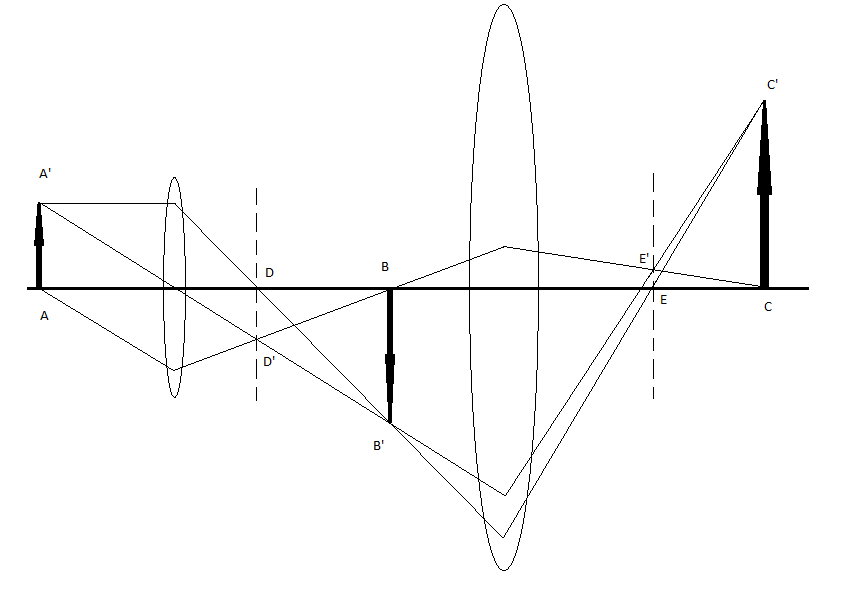
\includegraphics[width=\textwidth]{Strahlengang.png}
\caption{Schematische und vereinfachte Darstellung des Strahlenganges zur Entstehung der zwei Bildarten. Realbilder bei BB' und CC'. Beugungsbilder bei DD' und EE'.}
\label{Strahlengang}
\end{figure}
Werden Elektronen an den Atomen im Kristall gestreut, so ergibt sich eine vom Steuwinkel abhängige Intensitätsverteilung. Die Elektronen werden nach dem Bragg-Gesetz gestreut. Da die Winkel durch die kurze Wellenlänge der Elektronen jedoch sehr klein sind, kann der Bragg-Winkel genähert werden zu:
\begin{align}
2d\theta = n\lambda
\end{align}
Mit \(\lambda\) der Wellenlänge der Elektronen, \(d\) dem Abstand der Atome im Gitter und \(\theta\) dem Winkel des Elektronenstrahls zur Atomebene. Somit werden für jeden Gitterbaustein bestimmte Reflexe erwartet. Jedoch entstehen nicht von jedem Gitterbaustein Reflexe. Über den Strukturfaktor können nun die verbotenen und erlaubten Reflexe, berechnet werden.
\begin{align}
F_\mathrm{hkl}= \sum_{j=1}^n f_\mathrm{j}(\theta)\exp[-2\pi i (hu_\mathrm{j}+kv_\mathrm{j}+lw_\mathrm{j})]
\end{align}
Mit \(h,k,l\) den Millerschen Indizes, \(f_\mathrm{j}(\theta)\) dem Streufaktor und \(j=1,2,3,...,n\) dem \(j\)ten Atom in der Einheitszelle am Ort \((u,v,w)\).\\
Das Ergebnis sind Beugungsbilder, die von der Kristallstruktur abhängig sind. Besteht eine Probe aus mehreren Kristallen mit unterschiedlicher Orientierung zueinander, so überlagern sich die jeweiligen Beugungsbilder.
Eine anschauliche Verdeutlichung des Bragg-Gesetzes ist die Ewald-Kugel (Abb. \ref{ewald}). Dabei wird in das reziproke Gitter des Kristalls der einfallende Elektronenstrahl mit der Länge \(1/\lambda\) auf einen gewählten Ursprungsreflex gezeichnet. Die Länge des Elektronenstrahls gibt den Radius eines Kreises, dessen Mittelpunkt der Anfang des Elektronenstrahls definiert. Alle Reflexe, die nun auf dem Kreis liegen, sind im Beugungsbild erkennbar. Da die Intensitätsbreite des Bragg-Winkels von der Dicke der Probe mit \(1/t\) abhängt, weicht das reziproke Gitter auf und es sind keine Punkte mehr, sondern Linien. Somit sind auch Relfexe sichtbar, wenn die Ewaldkugel knapp die reziproken Gitterpunkte verfehlt.
\begin{figure}\center
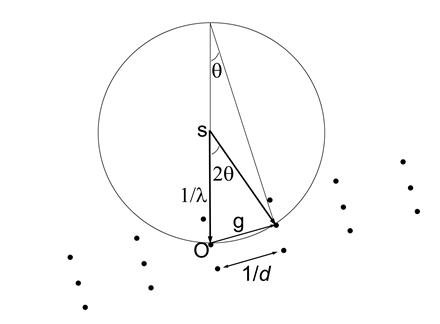
\includegraphics[width=0.65\textwidth]{ewald.png}
\caption{Konstruktion der Ewaldkugel im reziproken Kristallgitter.}
\label{ewald}
\end{figure}
	
\section{Versuchsaufbau und Versuchsdurchführung}
Bei dem verwendeten Transmissionselektronenmikroskop handelt es sich um ein Titan 80/300. Es wird verwendet um an einer InGaAs/GaAs-Probe Beugungs- und Realbilder aufzunehmen. Die Probe wurde im FIB präpariert und auf eine Dicke von wenigen Nanometern geschnitten. Im TEM werden in einer Kathode Elektronen freigesetzt und mittels einer an die Lochanode angelegte Spannung von \(300\,\mathrm{kV}\) beschleunigt (Abb \ref{TEM}). Über ein System aus elektromagnetische Linsen werden die Elektronen auf die Probe fokussiert. Dort werden die Elektronen teilweise an den Atomen im Kristallgitter gestreut nach dem Bragg-Gesetz und teilweise reflektiert. Auch werden Elektronen aus den inneren Energieniveaus herausgeschlagen. Wodurch Elektronen aus höheren Energieniveaus in das entstandene Loch zurückfallen und ihre überschüssige Energie als elektromagnetische Strahlung abgeben. Dies ist die charakteristische Röntgenstrahlung und kann auch über ein EDX-System analysiert werden. Dies erlaubt die Bestimmung des Materials.
Die gestreuten Elektronen werden transmittiert und werden wiederum über ein Linsensystem fokussiert. Die Elektronen treffen nun auf einen Beobachtungsschirm, oder eine CCD-Kamera. Über eine weitere Linse wird nun der Strahlengang so gelegt, dass entweder das Beugungsbild, oder das Abbildungsbild zuerkennen ist. Der gesamte Strahlengang befindet sich im Hochvakuum, sodass unerwünschte Wechselwirkungen der Elektronen mit der Luft verhindert werden.
\begin{figure}[H]
\center
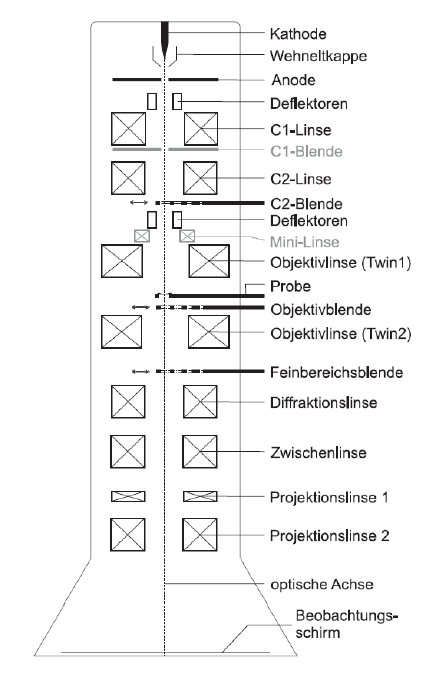
\includegraphics[width=0.6\textwidth]{tem.png}
\caption{schematischer Aufbau eines Transmissionselektronenmikroskop. Die aus der Kathode beschleunigten Elektronen werden über mehrere Linsen- und Blendensysteme auf die Probe fokussiert. Nach der Transmission werden die Elektronen erneut auf einen Beobachtunsschirm, oder eine Kamera fokussiert.}
\label{TEM}
\end{figure}
Bevor das Beugungsbild einer Probe aufgenommen werden kann, muss das TEM zuerst justiert werden. Dazu wird der Elektronenstrahl auf das Vakuum fokussiert. Als erstes wird die C2-Blende zentriert, sodass bei einem Vergrößerungswechsel der Strahl in der Mitte des Schirms bleibt. Danach wird der Elektronenstrahl auf eine kreisrunde Form gebracht, da dieser durch den Kondensorastigmatismus zumeist elliptische ist. Als dritter Schritt wird der Strahl auf die Probenoberfläche fokussiert und anschließend wird das Rotationszentrum durch verkippen der Probe eingestellt. Nach der Justage werden Beugungsbilder aufgenommen, sowohl in Zonenachse, als auch mit anderen Lauekreiszentren. Danach werden Aufnahmen im Abbildungsmodus gemacht, wobei Hellfeld-, aber auch Dunkelfeldaufnahmen mit den Reflexen (022) und (004) gemacht werden. Auf der InGaAs/GaAs-Probe befinden sich InGaAs-Quantentrögen, von denen Aufnahmen gemacht werden, um im Anschluss einmal über den Gitterabstand und einmal über den Intensitätsverlauf den Indiumgehalt zubestimmen.

\section{Auswertung}

Es wurde eine GaAs Probe untersucht, die Quantentröge aus InGaAs enthält. Auf einem Bereich mit mehreren solchen Quantentrögen wurde das Beugungsbild in Abb. \ref{100ind} aufgenommen, während die Probe in Zonenachse [100] orientiert war.

\begin{figure}[h]\centering
	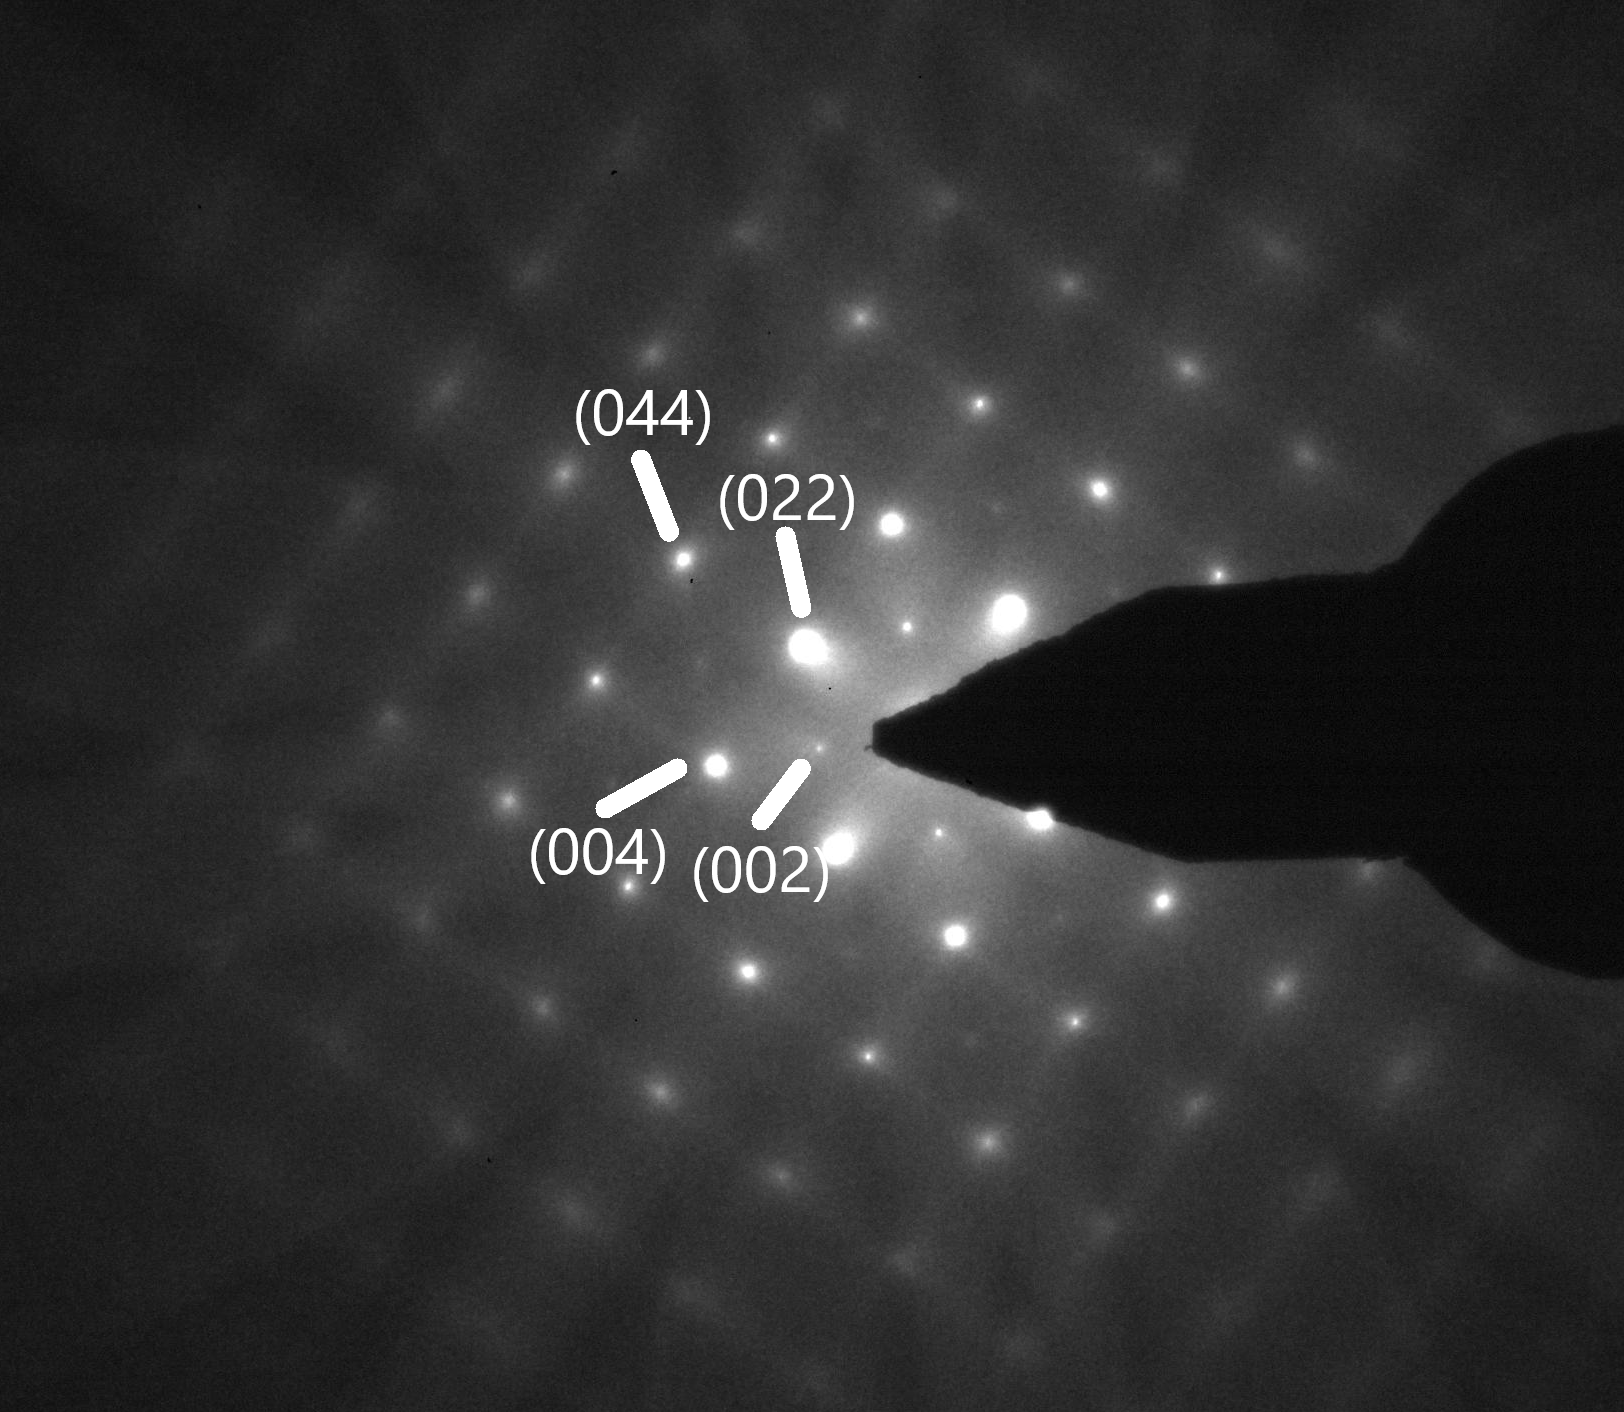
\includegraphics[width=0.65\textwidth]{Versuchsdaten/8/indiziert2.png}
\label{100ind}
\caption{Beugungsbild auf InGaAs in Zonenache [100]}
\end{figure}

Die Zonenachse [100] ist dadurch zu erkennen, dass die Intensitäten der Reflexe symmetrisch um den Punkt (000) verteilt sind. Wird die Probe verkippt, bilden sich Lauekreise mit Zentren abseits des Punktes (000), sodass der Punkt (000) immer auf dem Rand des Kreises liegt. Da GaAs ein Kubisches Gitter mit zwei Atomsorten bildet, haben alle Punkte mit ungeraden Laue-Indizes einen Strukturfaktor von 0. Dementsprechend sind die entsprechenden Reflexe auf dem Beugungsbild auch nicht zu erkennen.
Im Folgenden wurden mehrere Beugungsbilder mit unterschiedlichen Lauekreiszentren aufgenommen.

\begin{figure}[htb]\centering
	\subcaptionbox{Beugungsbild mit Lauekreiszentrum (008)\label{008}}
	[.49\linewidth]{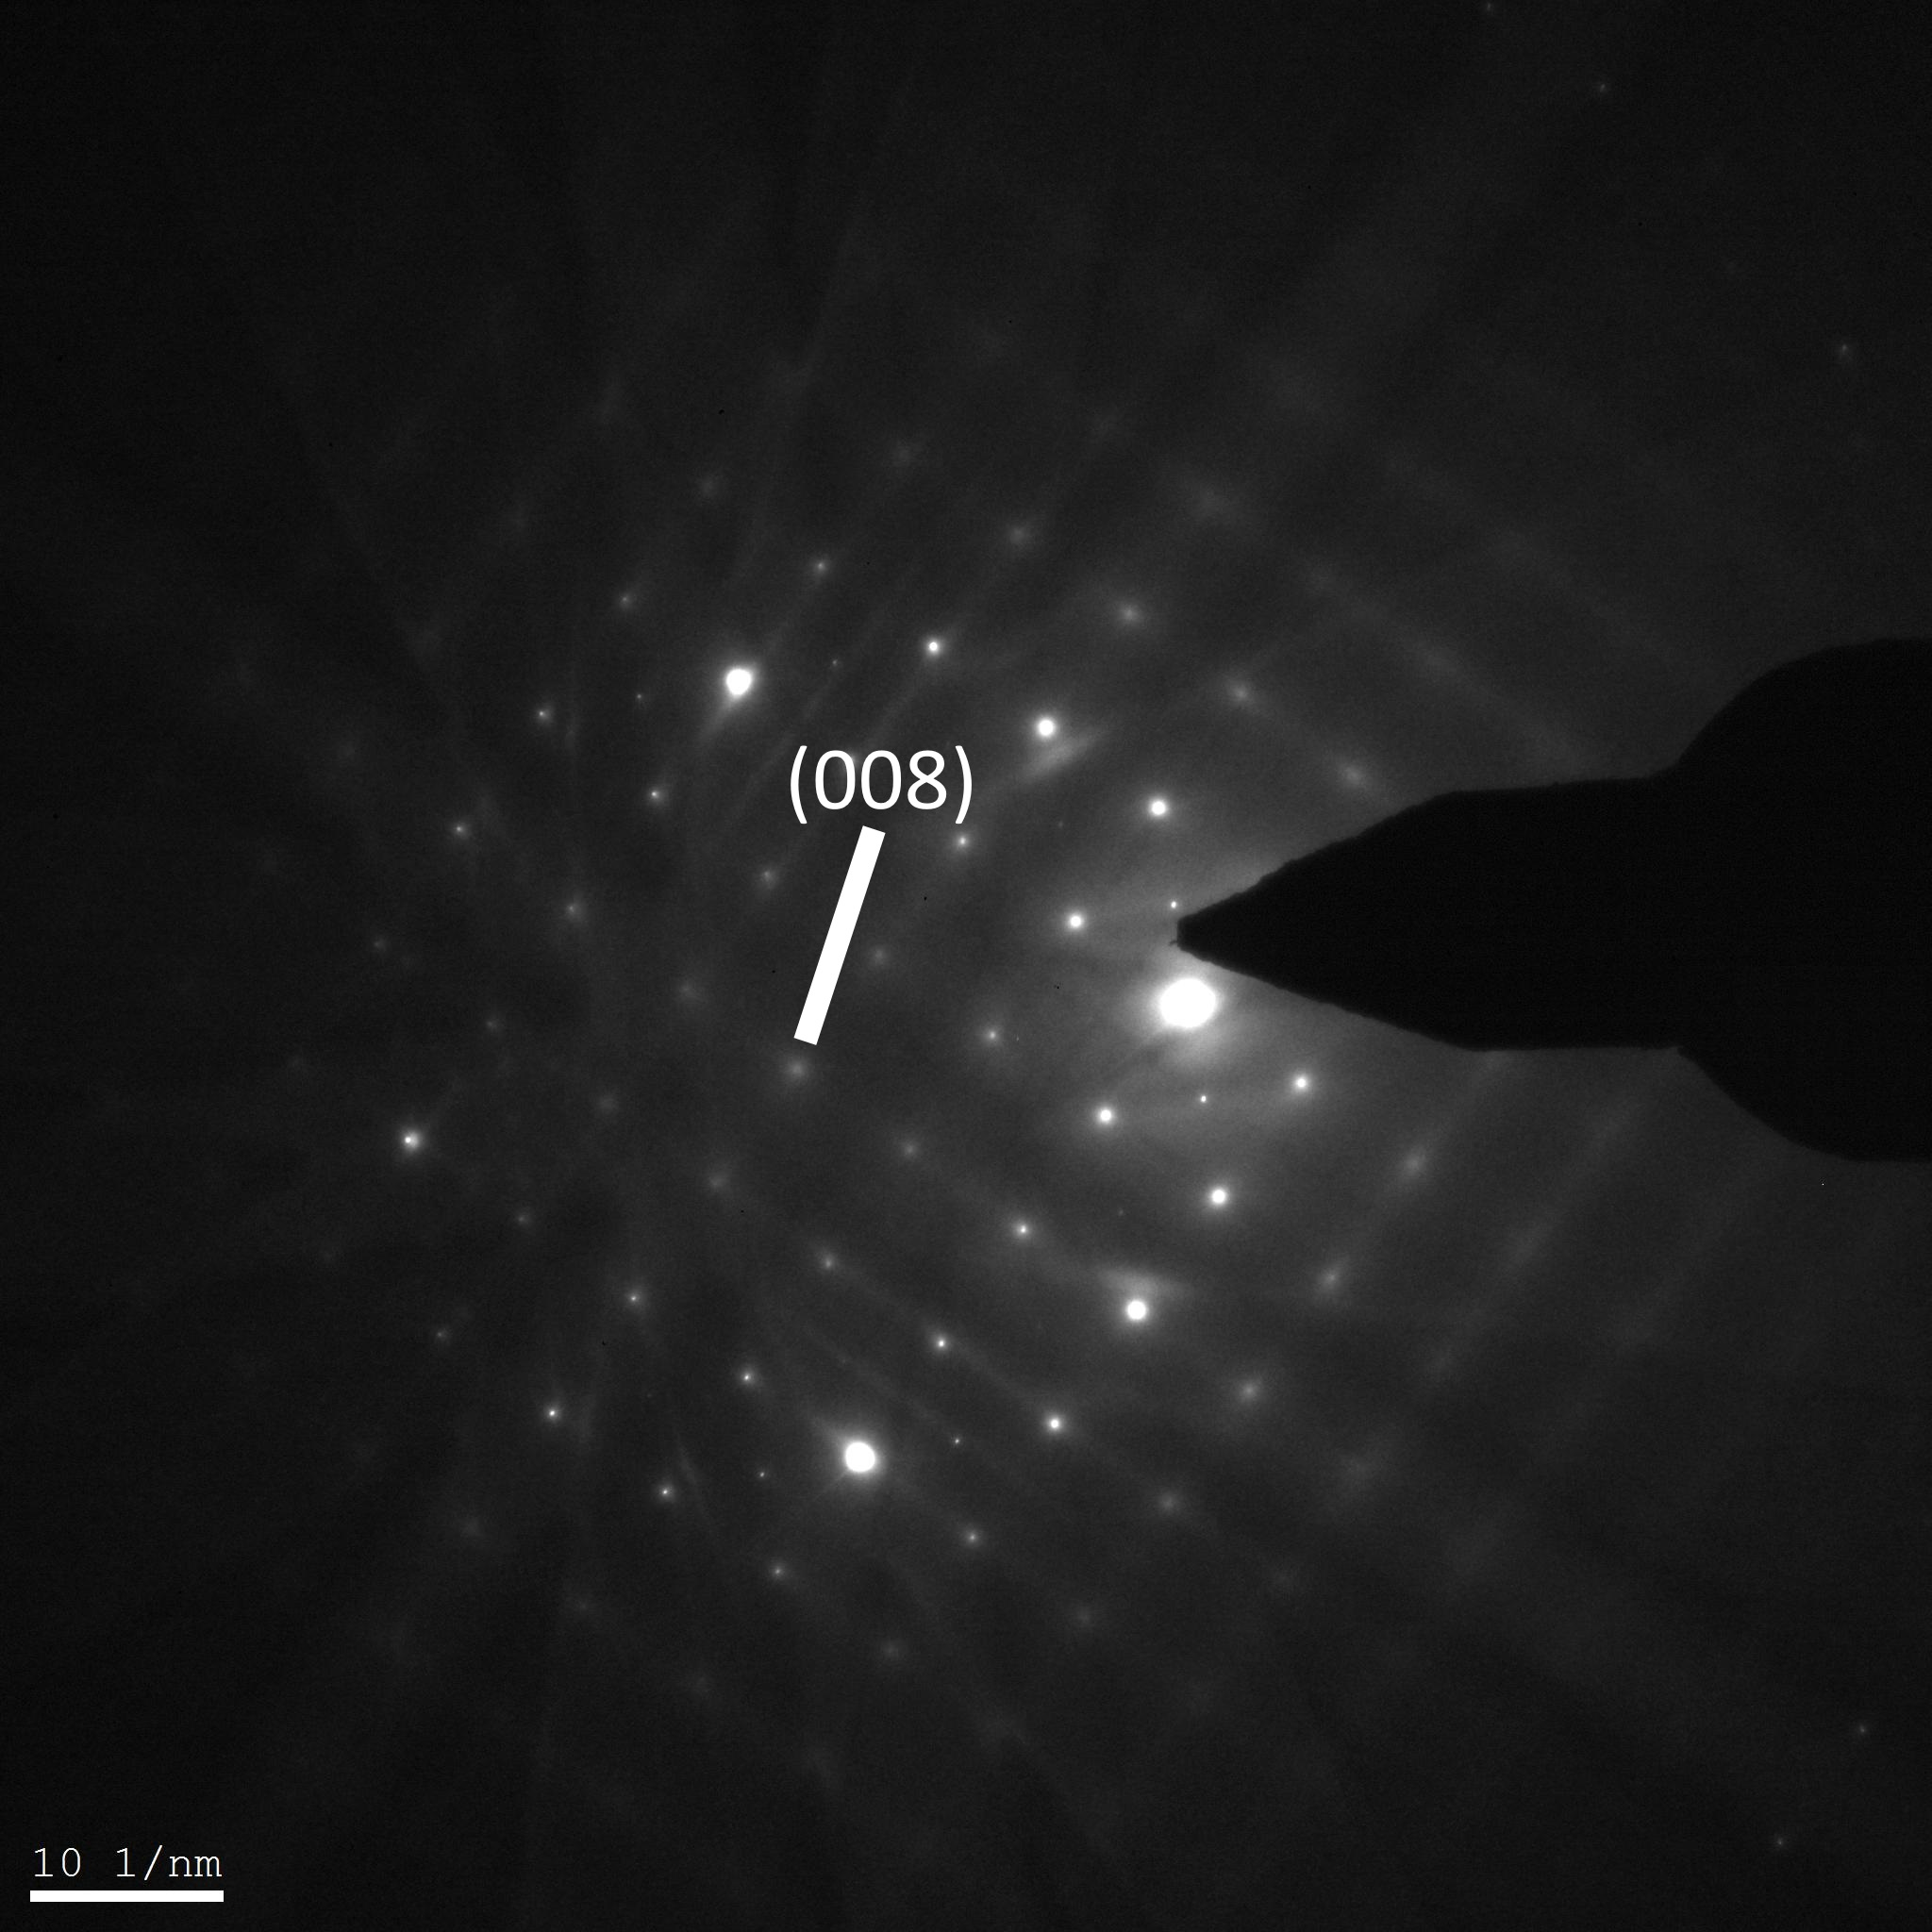
\includegraphics[width=0.49\textwidth]{Versuchsdaten/9/008.jpg}}
	\subcaptionbox{Beugungsbild mit Lauekreiszentrum (022)\label{022}}
	[.49\linewidth]{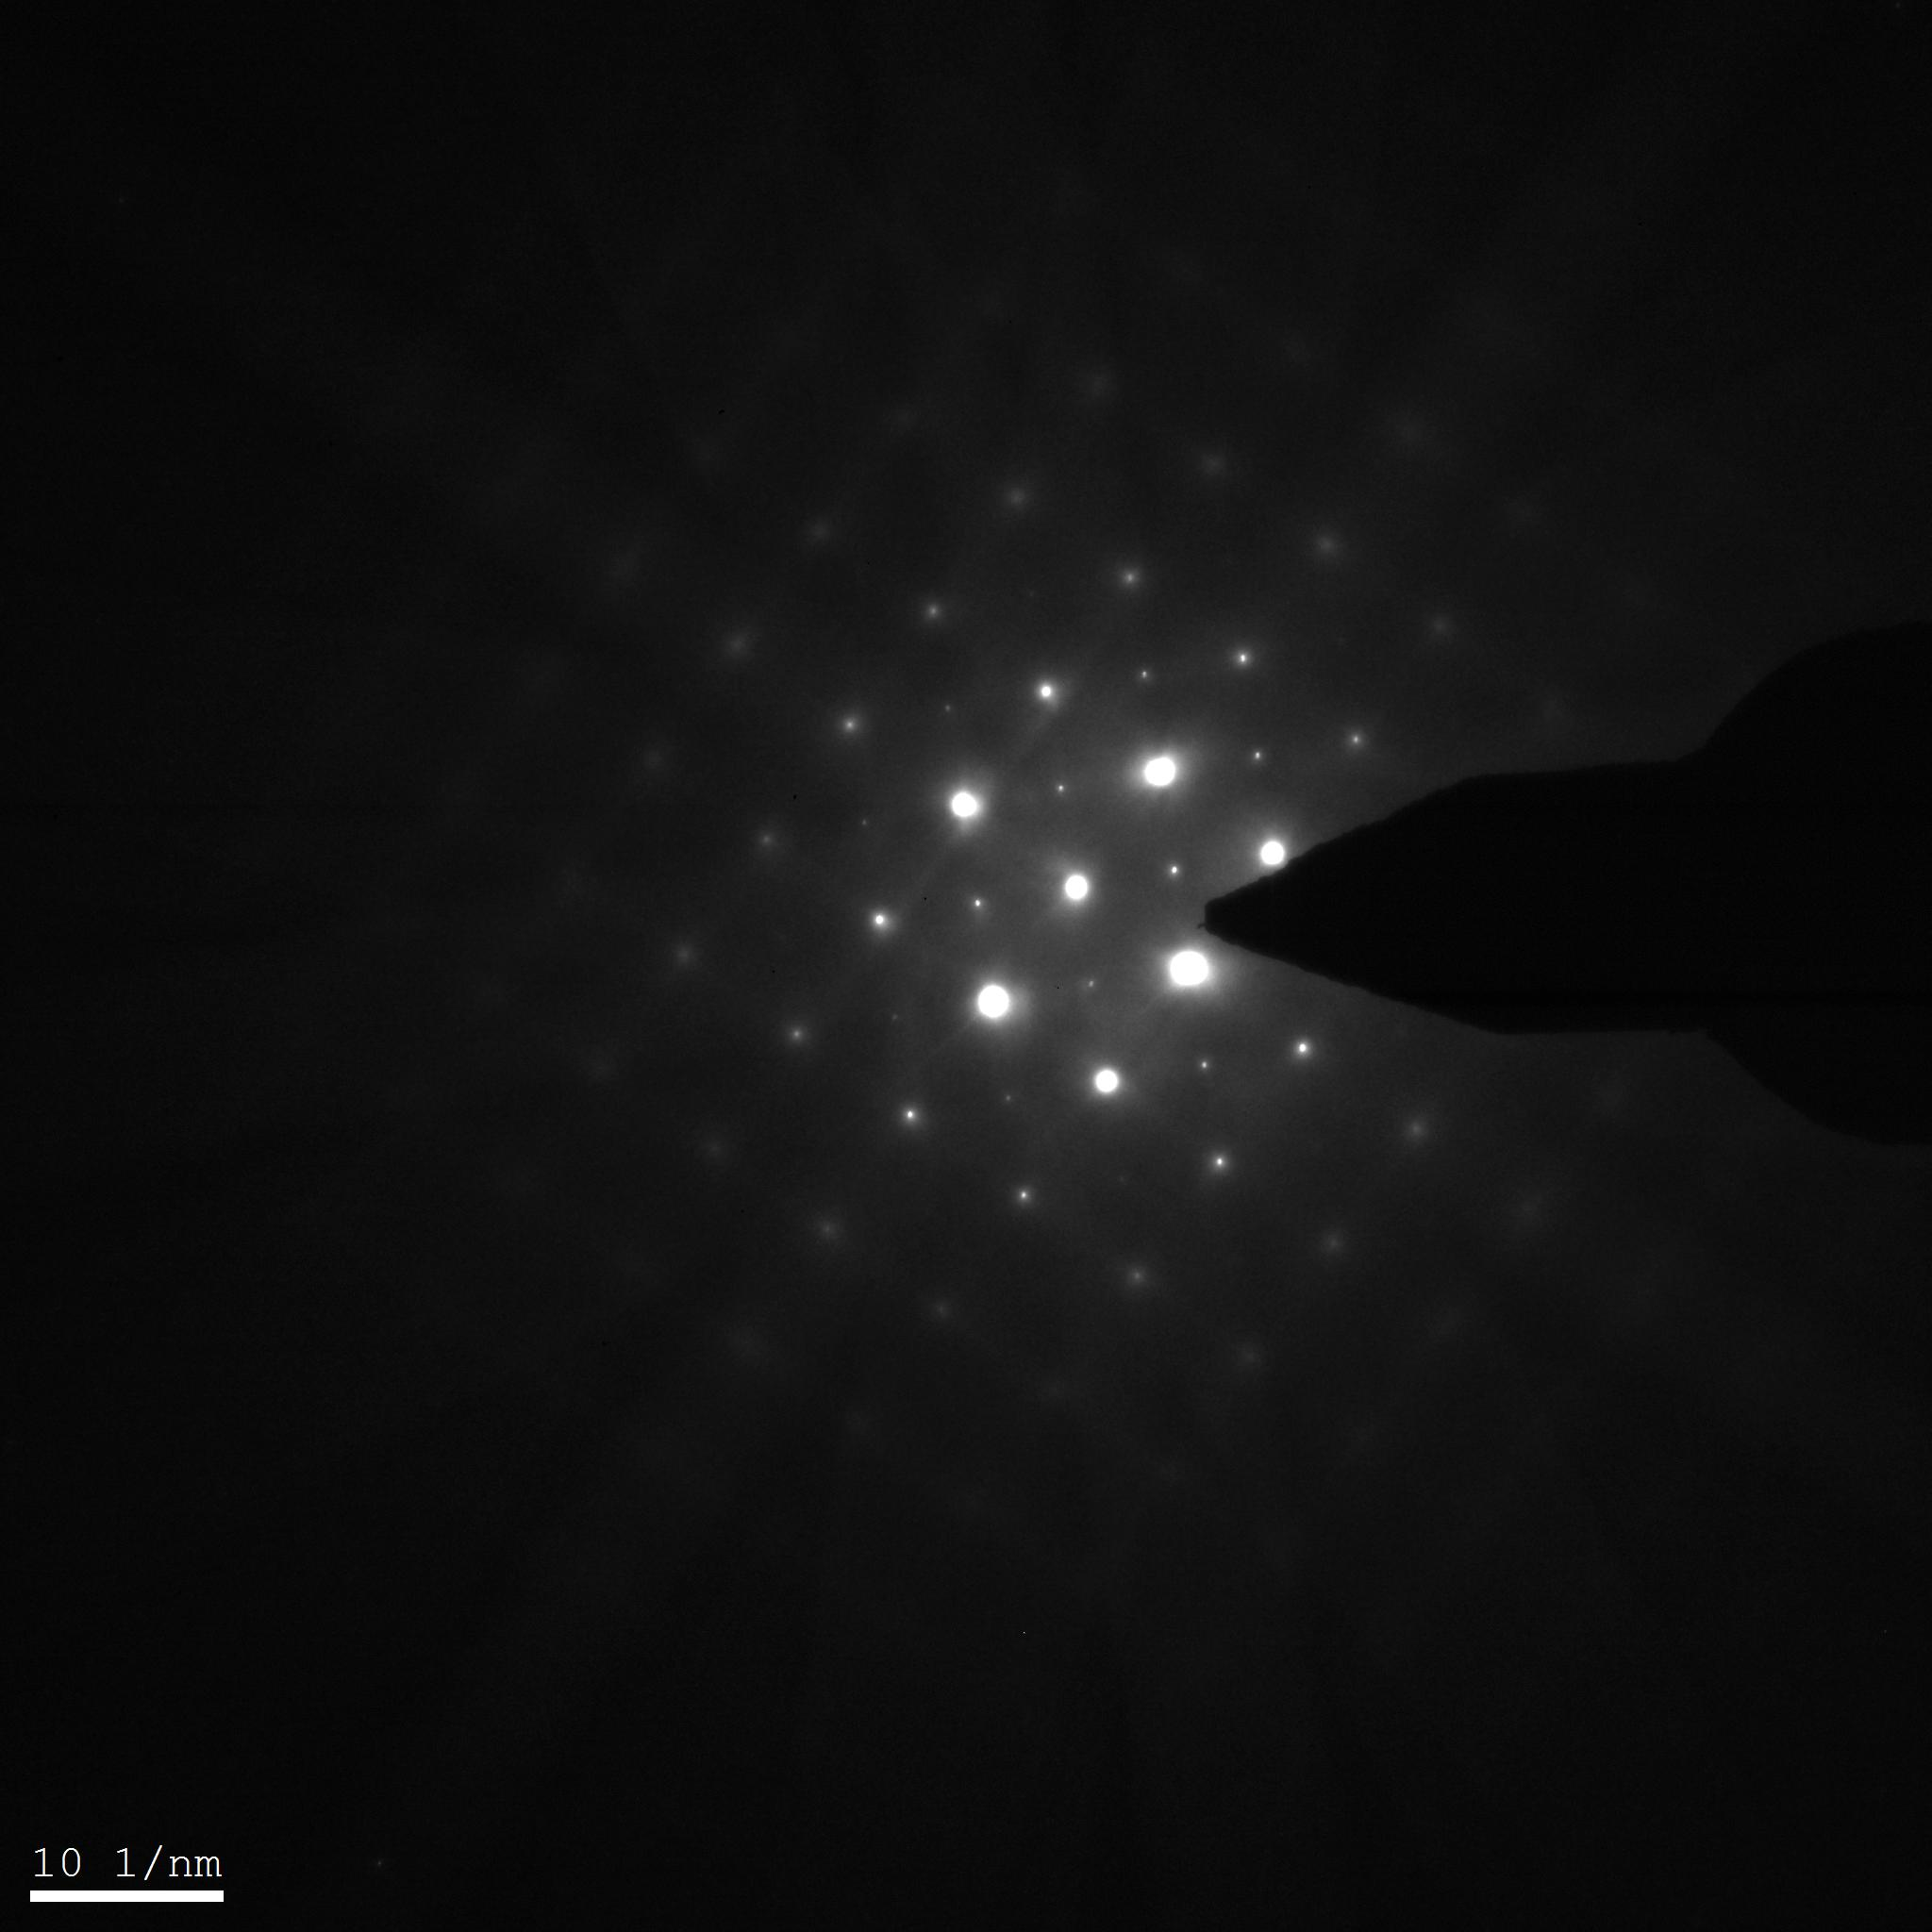
\includegraphics[width=0.49\textwidth]{Versuchsdaten/9/022.jpg}}\\
	\caption{Beugungsbilder bei unterschiedlichen Probendrehung} \label{laue1}
\end{figure}

In den Abb. \ref{008} und \ref{022} sind diese Beugungsbilder zu sehen. Im Lauekreis um das jeweilige Zentrum herum haben diejenigen Reflexe eine starke Intensität, die die Bragg-Reflexionsbedingung erfüllen. Eine Verschiebung des Lauekreiszentrums entsteht zudem auf unterschiedlichen Probenstellen durch geringe Unebenheiten oder auch durch anders ausgerichtete Kristallebenen erfolgen. \\
Damit die (004) Netzebenen in Bragg-Reflexionsstellung sind, muss der (004) Reflex im Beugungsbild auf dem Lauekreis liegen. Dies ist im einfachsten Fall beim Lauekreiszentrum (002) gegeben. Zu sehen ist dieser Fall in Abb. \ref{002} zu sehen.

\begin{figure}[h]\centering
	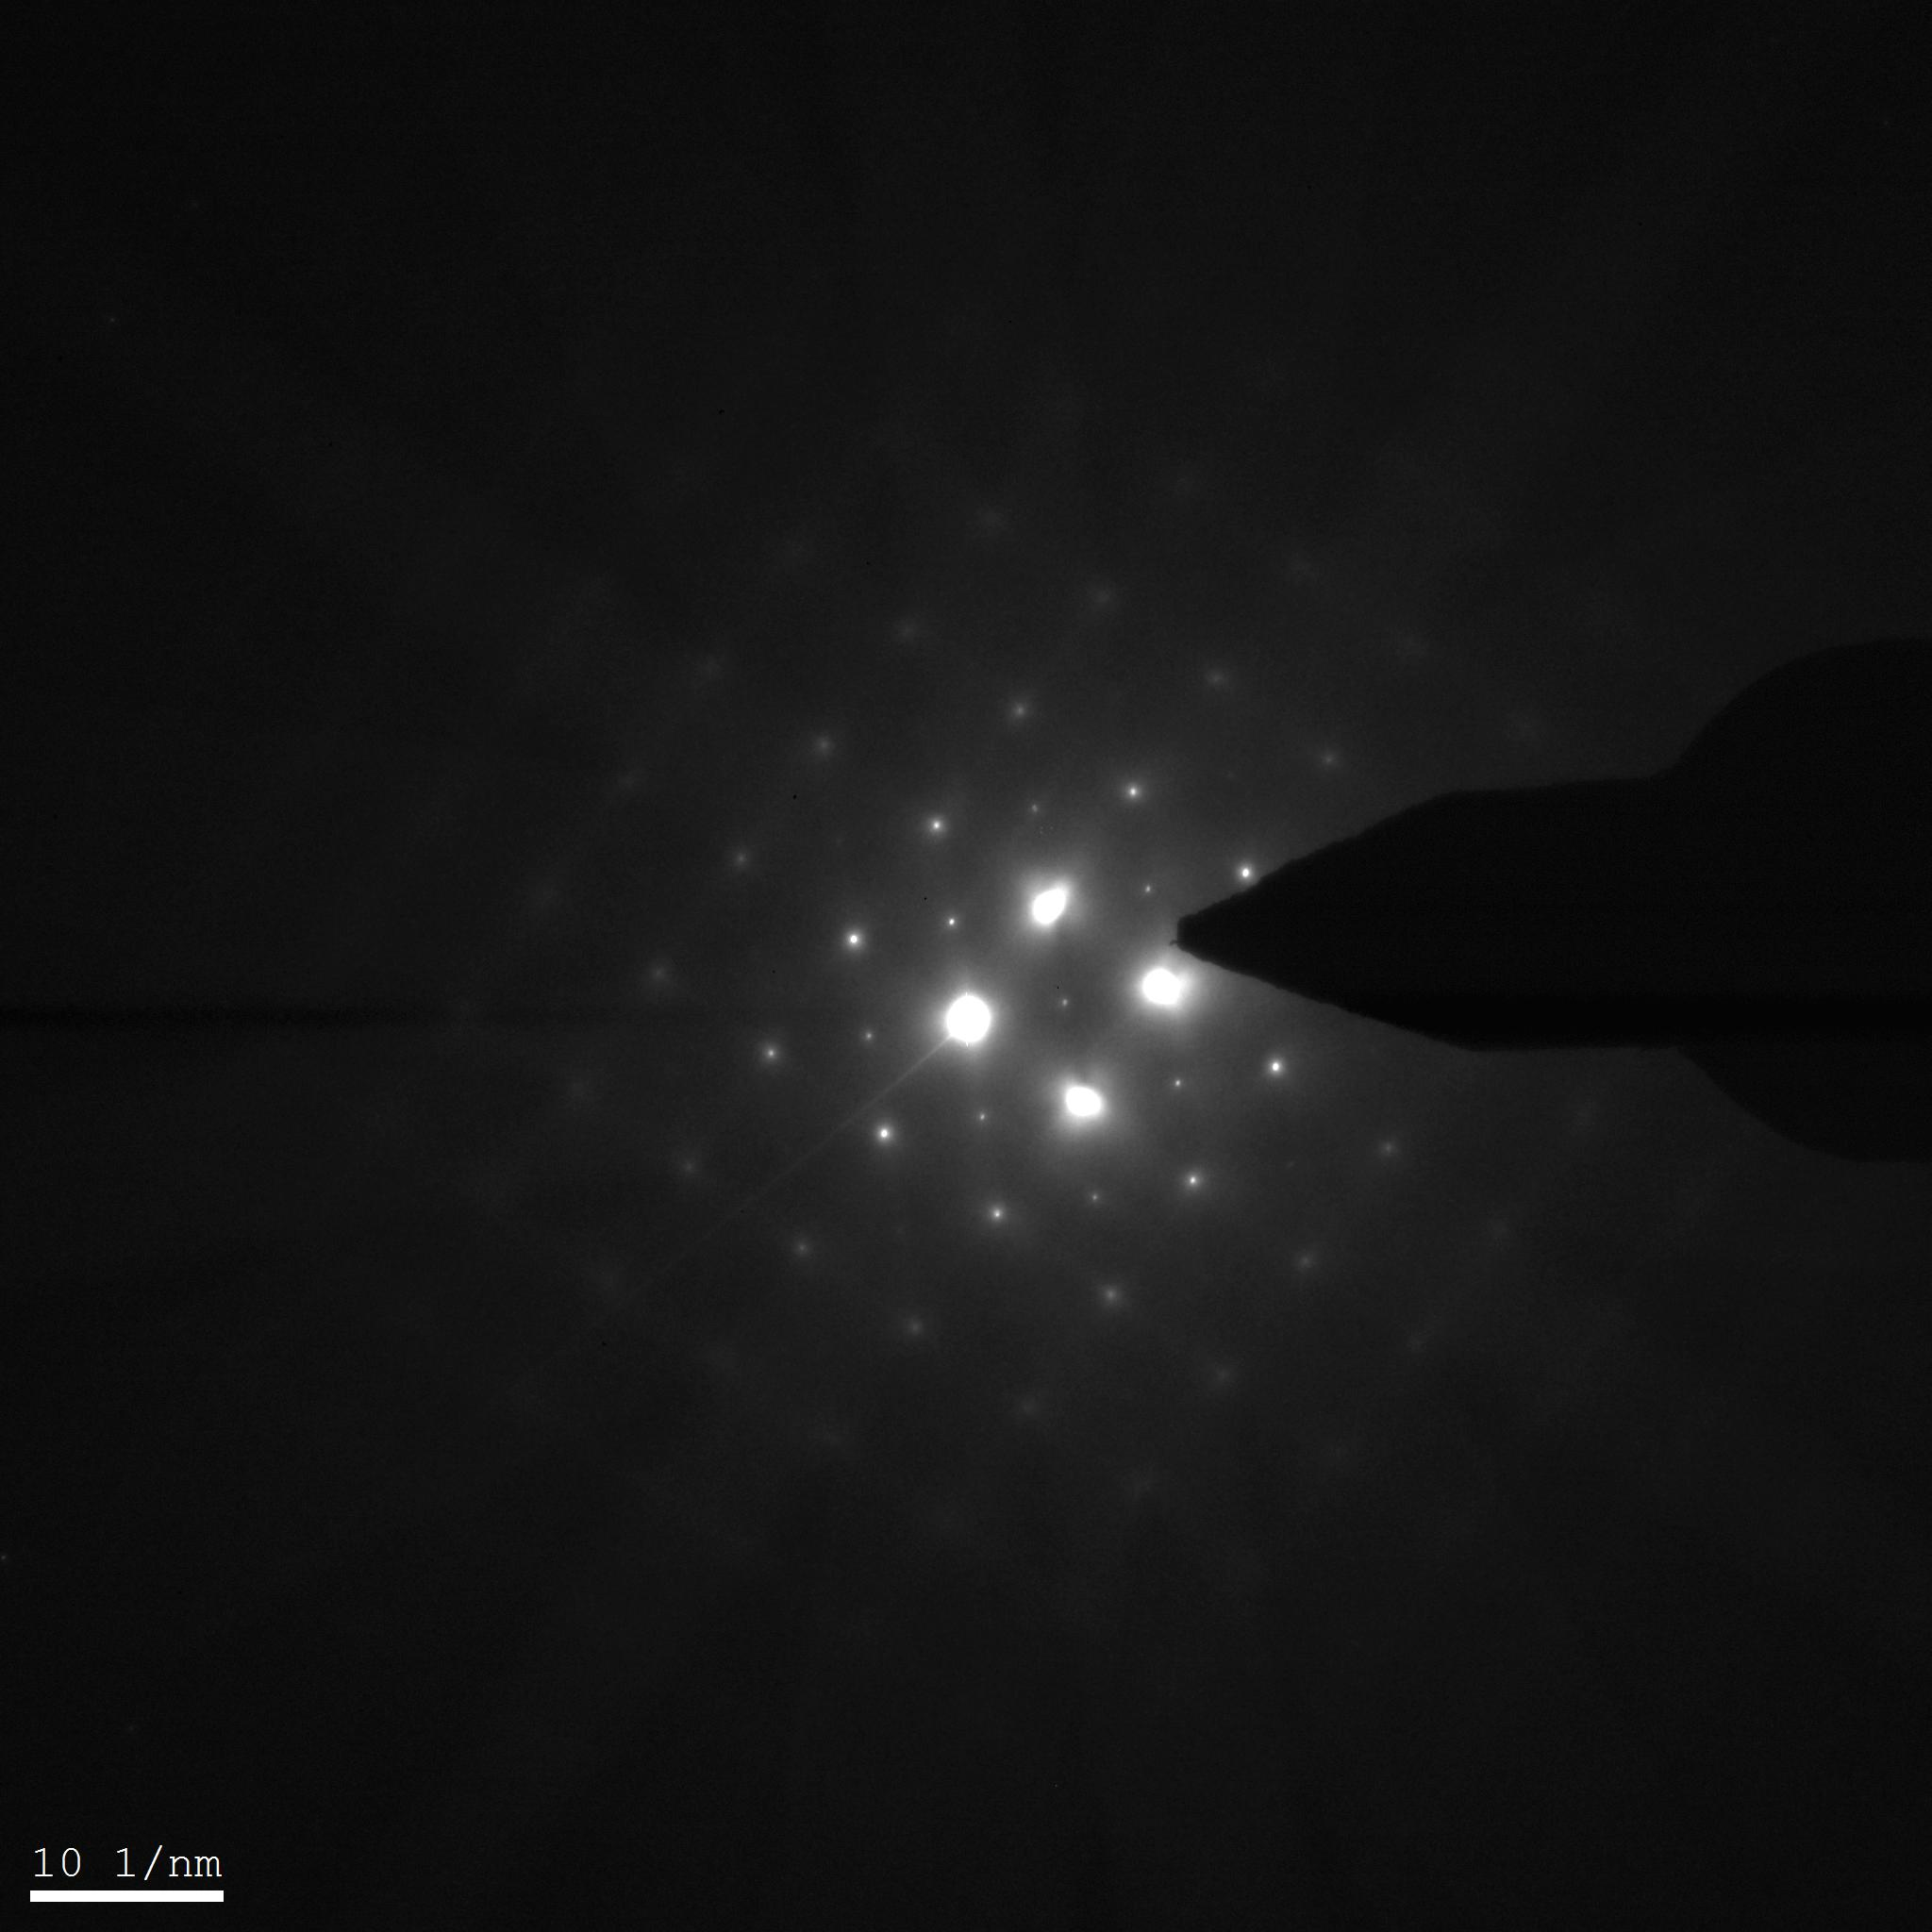
\includegraphics[width=0.65\textwidth]{Versuchsdaten/9/002.jpg}
\label{002}
\caption{Beugungsbild mit Lauekreiszentrum (002)}
\end{figure}

Zudem liegt der Reflex (022) in diesem Fall ebenfalls auf dem Lauekreis. Indem mit einer kleinen Blende alle Reflexe bis auf einen ausgeblendet werden, konnten im Folgenden Dunkelfeldaufnahmen der Probe gemacht werden.

\begin{figure}[htb]\centering
	\subcaptionbox{Hellfeldaufnahme\label{hell}}
	[.32\linewidth]{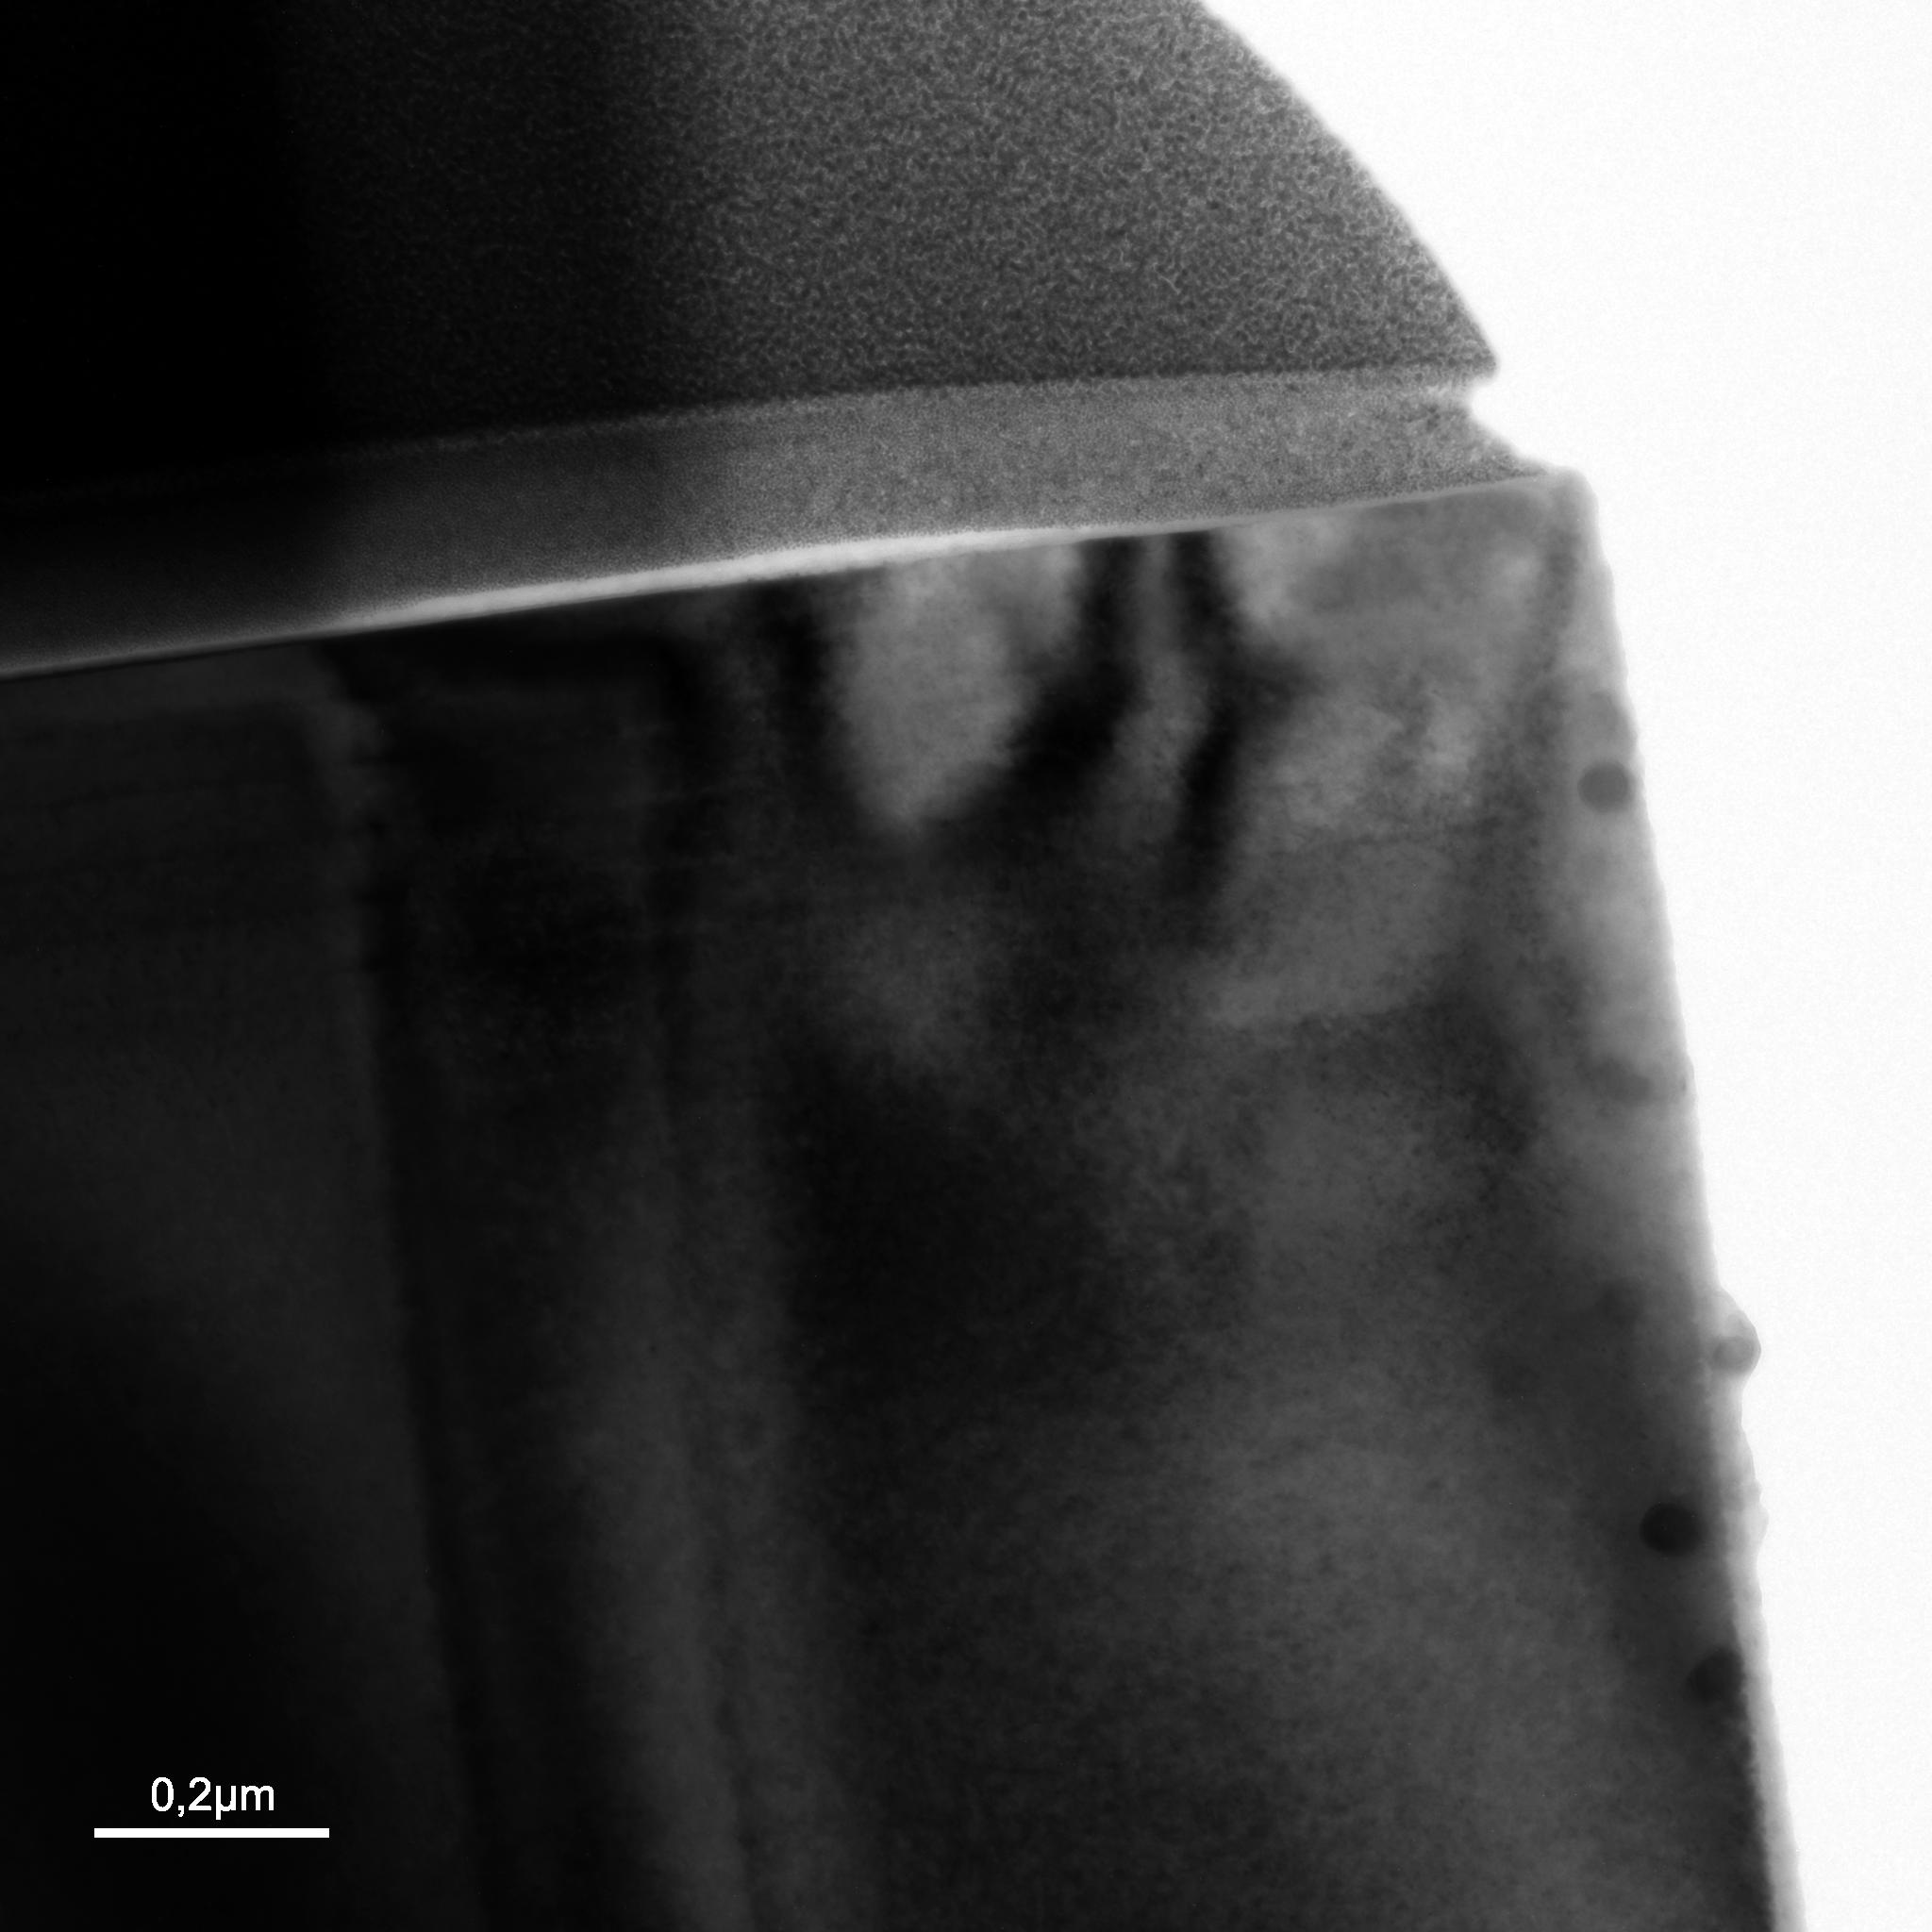
\includegraphics[width=0.32\textwidth]{Versuchsdaten/10/hell.jpg}}
	\subcaptionbox{Dunkelfeldaufnahme mit Reflex (004)\label{dunkel004}}
	[.32\linewidth]{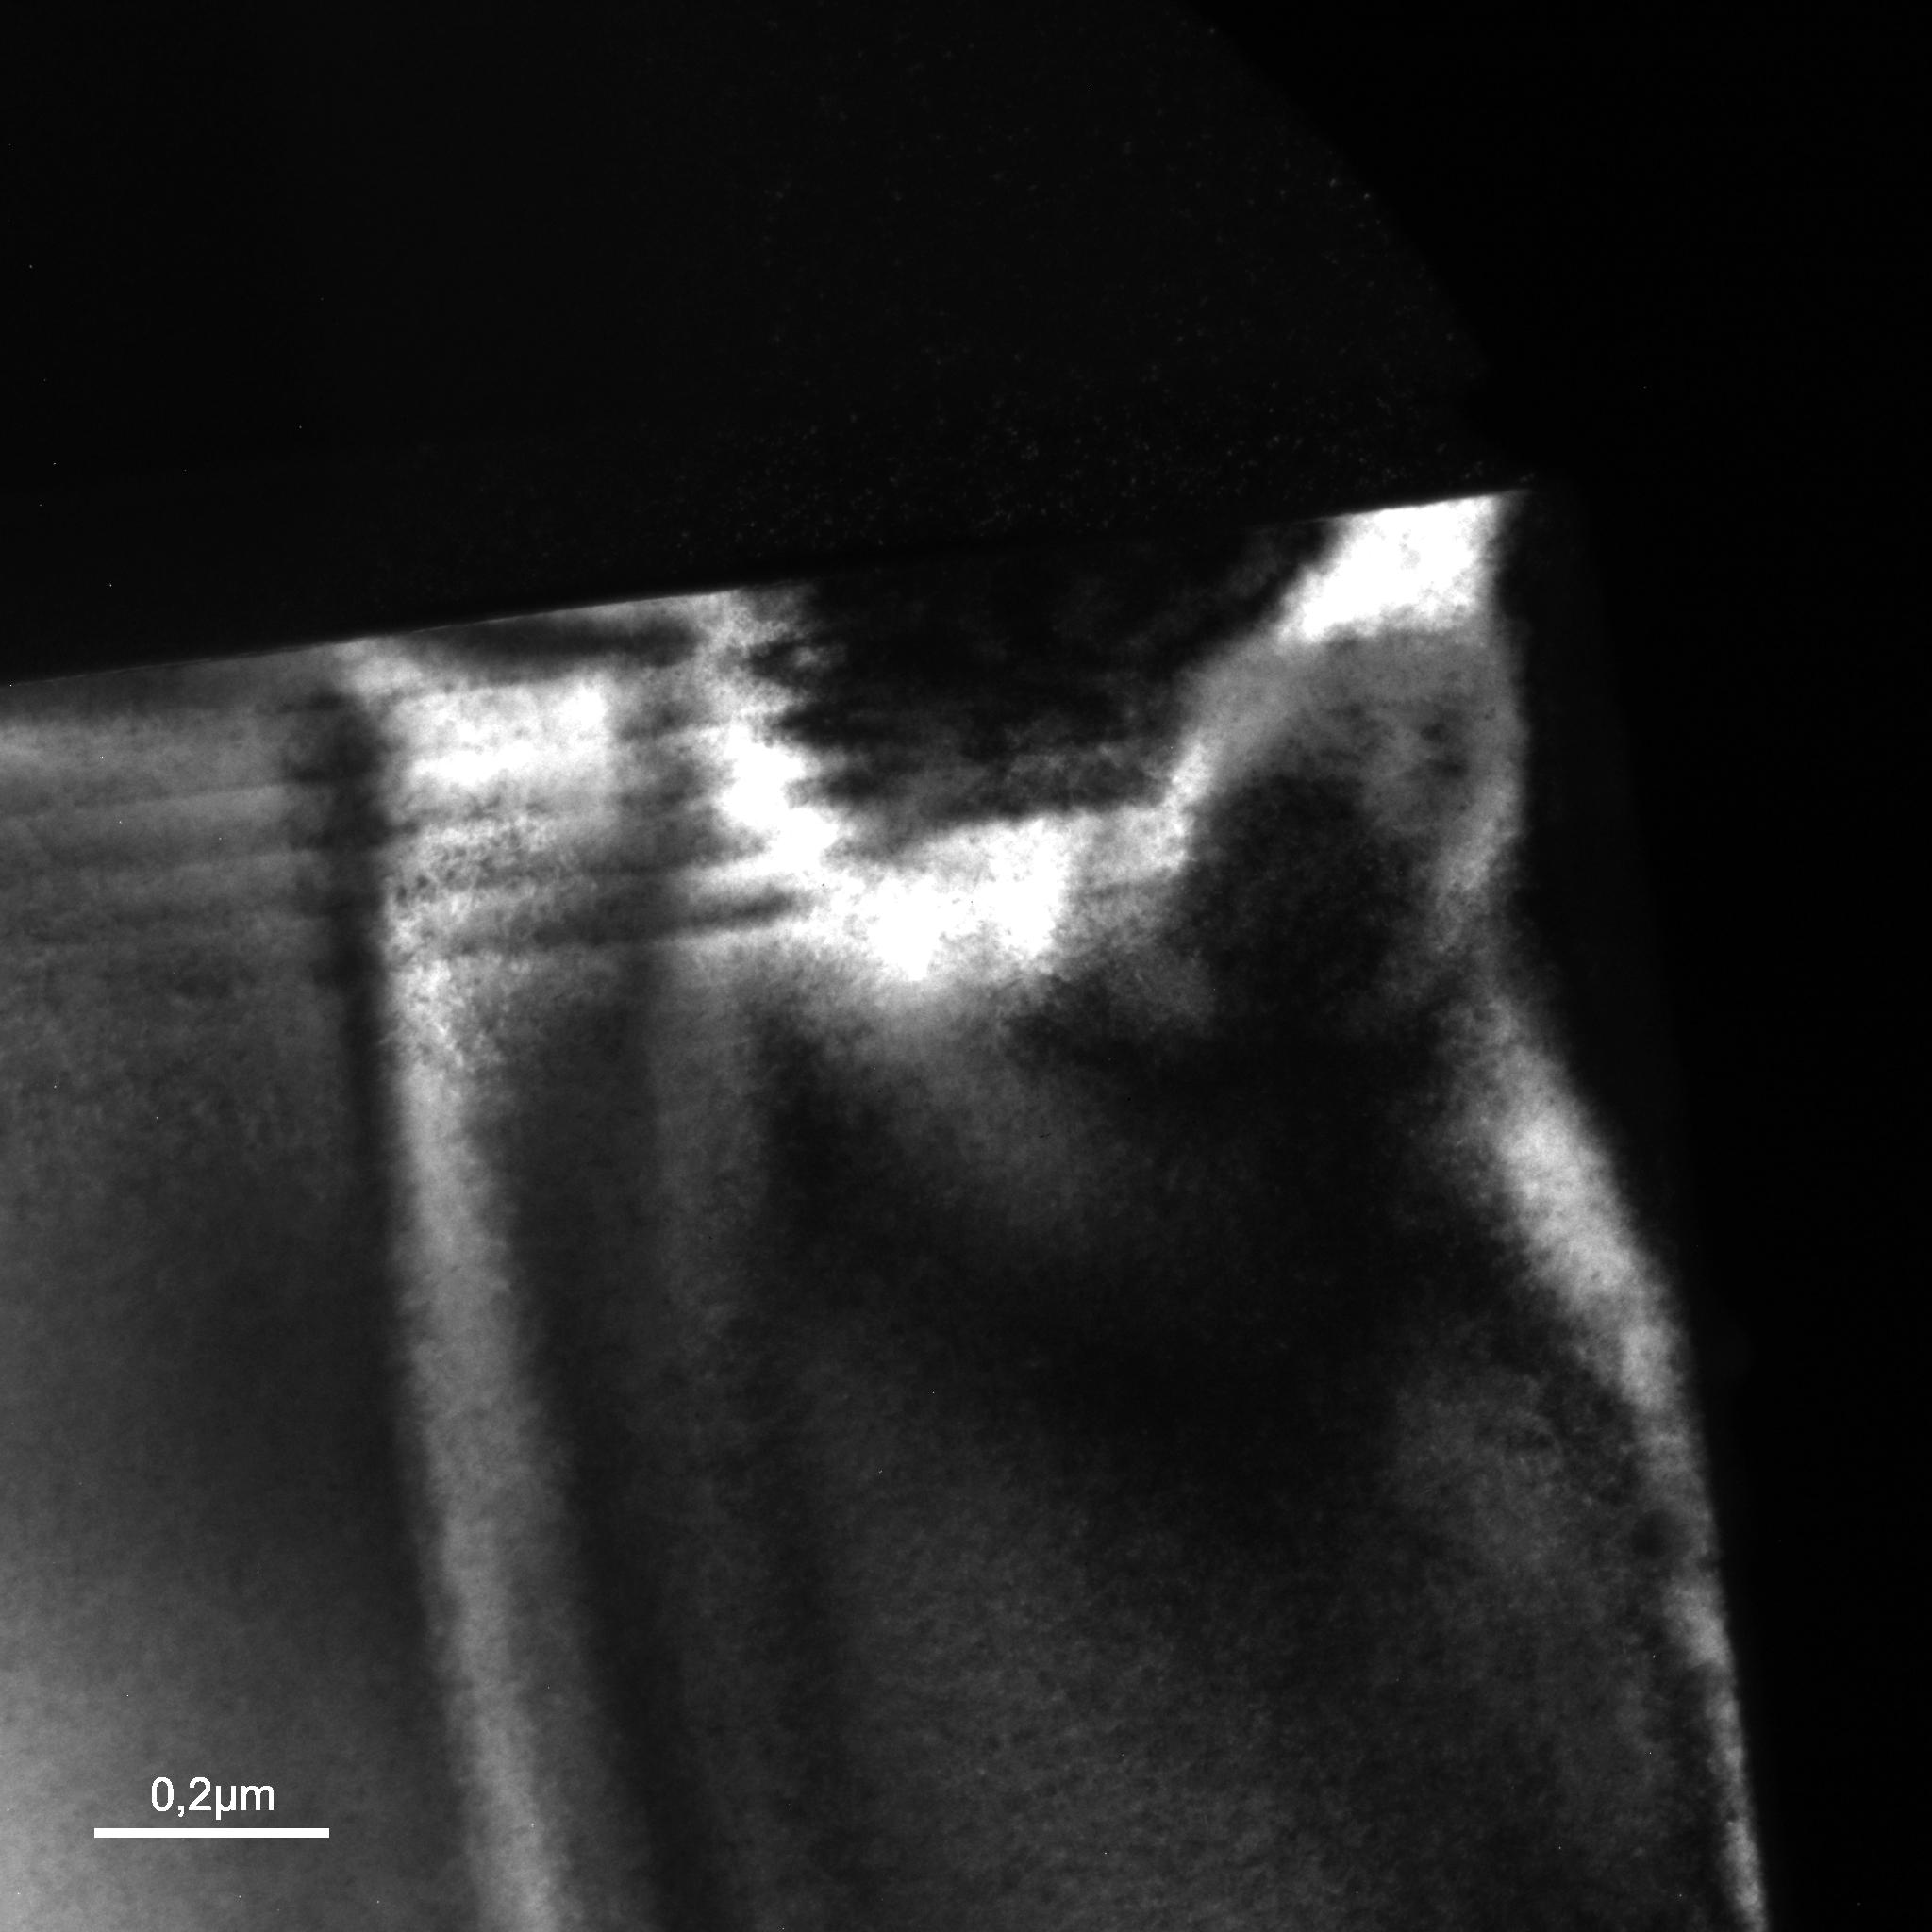
\includegraphics[width=0.32\textwidth]{Versuchsdaten/10/004-dunkel.jpg}}
	\subcaptionbox{Dunkelfeldaufnahme mit Reflex (022\label{dunkel022}}
	[.32\linewidth]{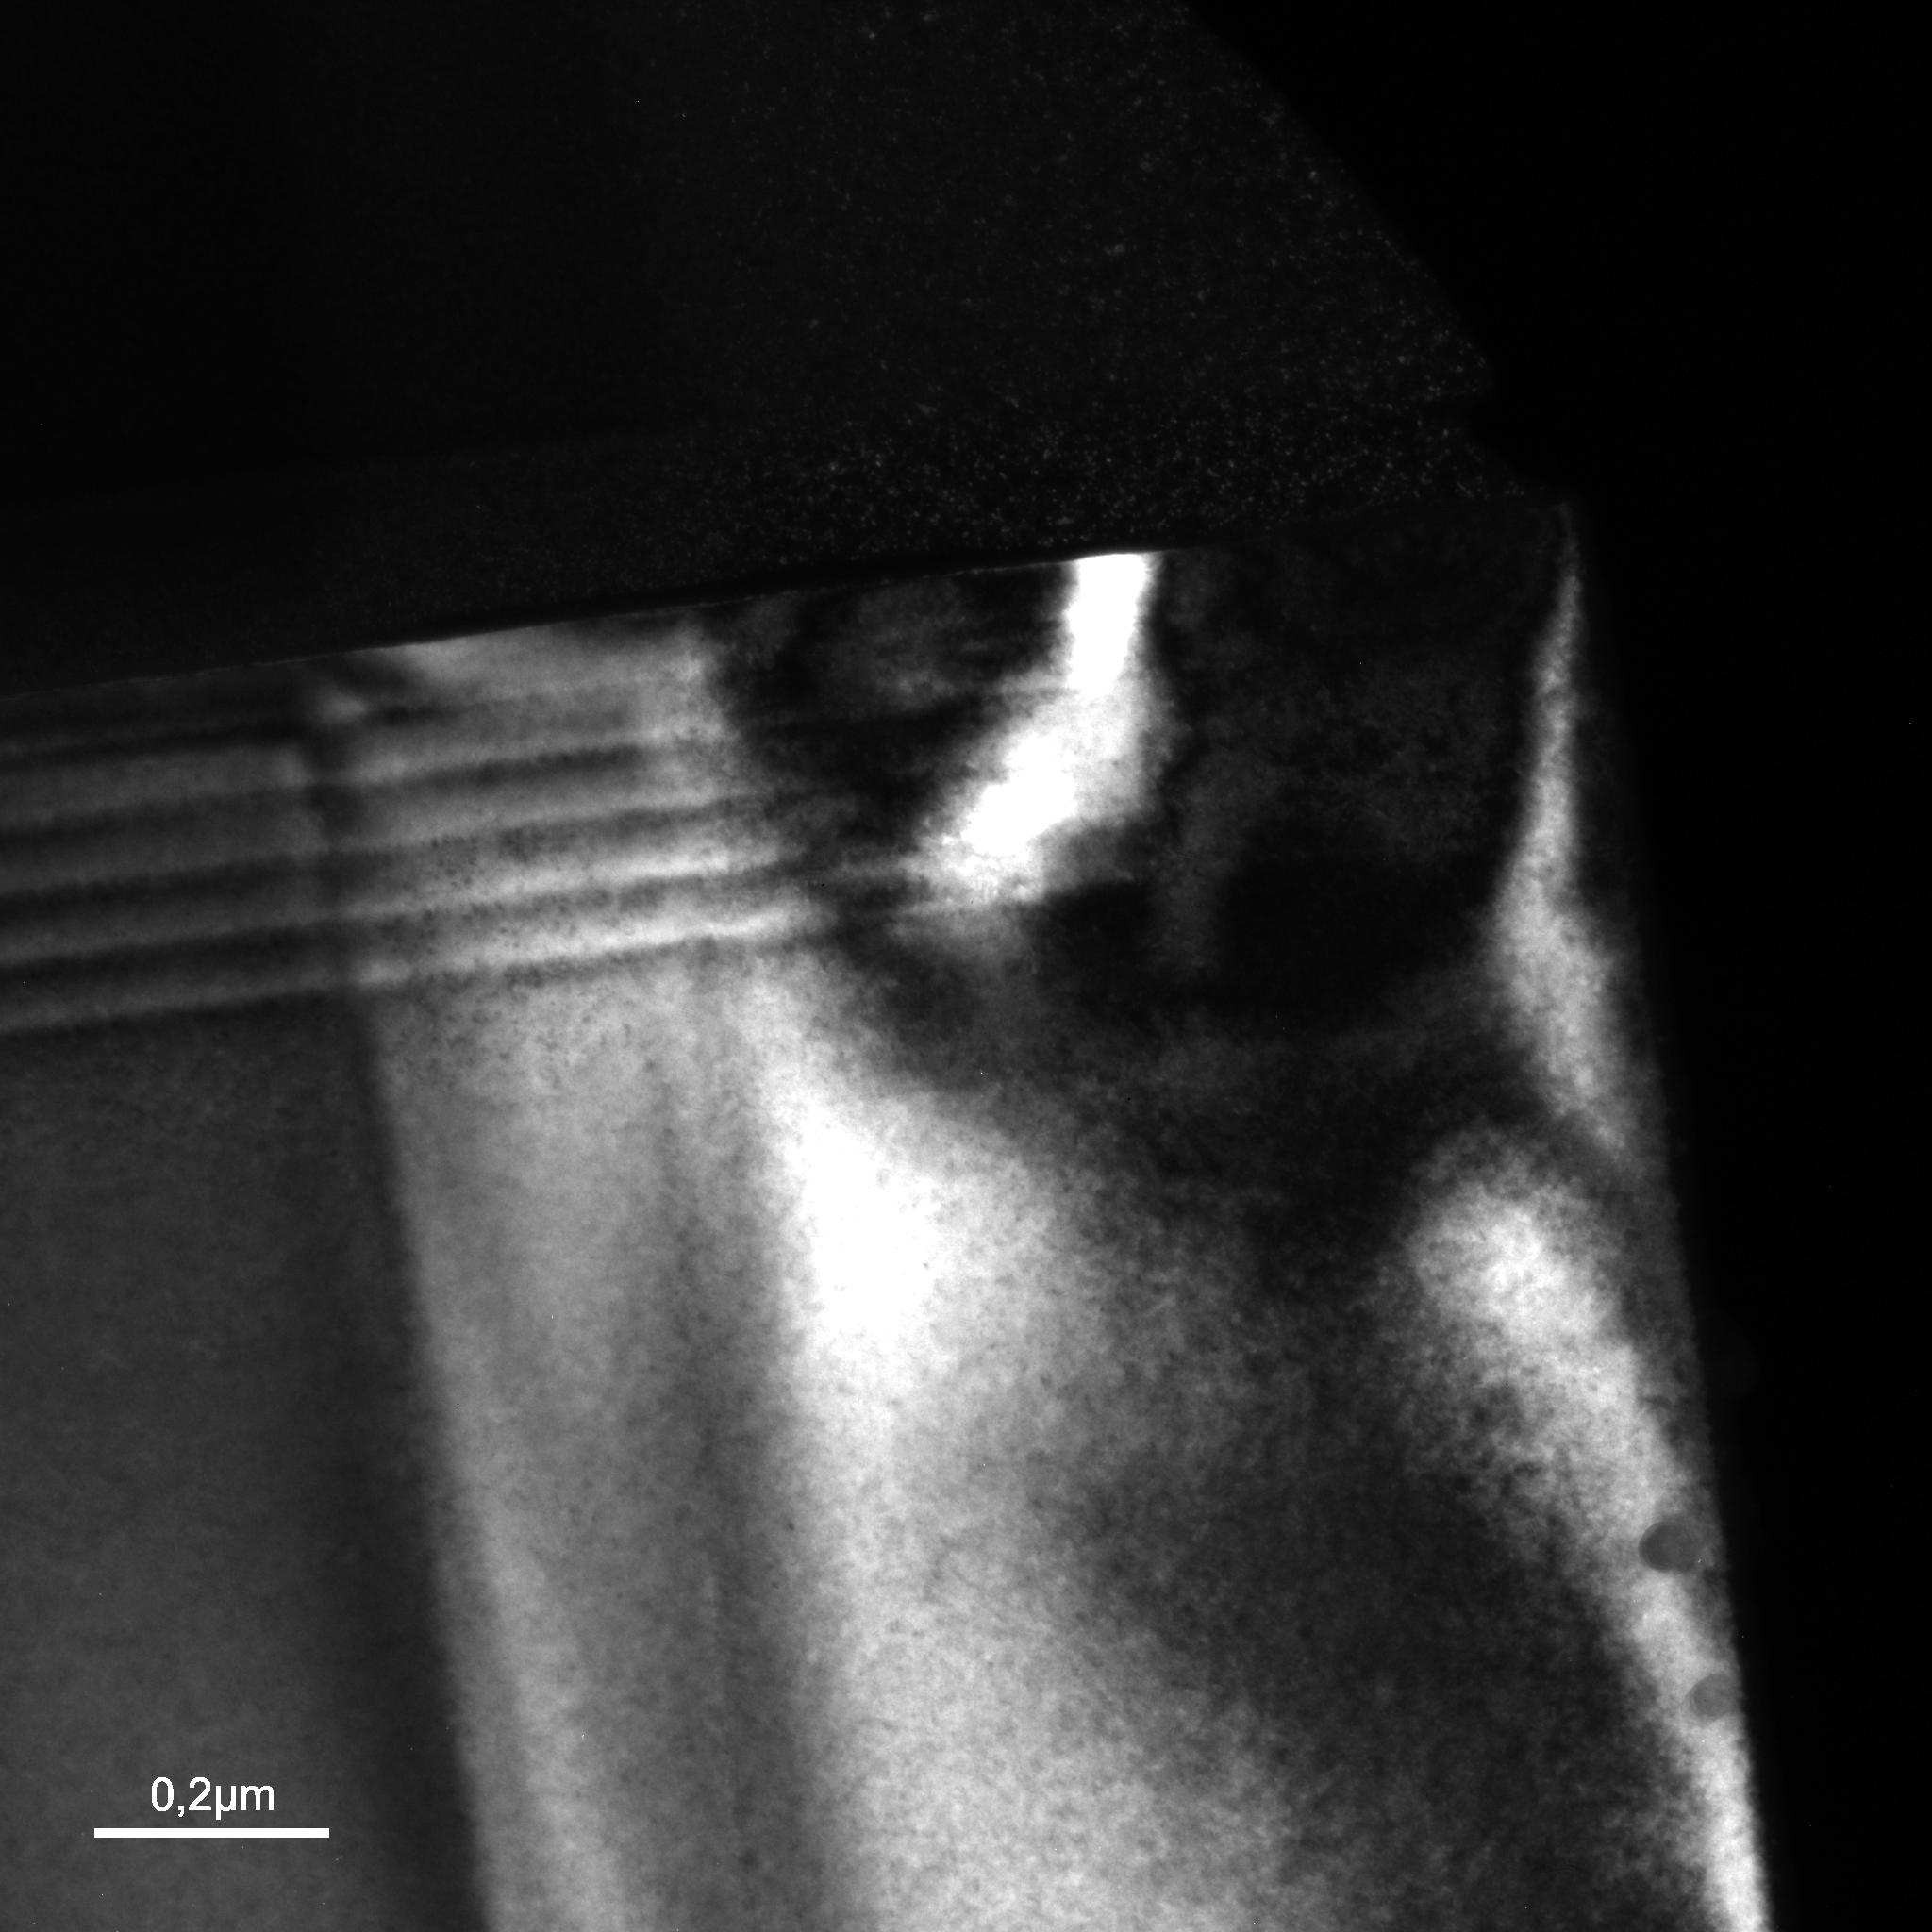
\includegraphics[width=0.32\textwidth]{Versuchsdaten/10/022-dunkel.jpg}}
	\caption{Aufnahmen der InGaAs Quantentröge} \label{dunkelhell}
\end{figure}

Zum Vergleich ist in Abb. \ref{hell} eine Hellfeldaufnahme der Probenstelle zu sehen. In den Abb. \ref{dunkel004} und \ref{dunkel022} sind zwei Dunkelfeldaufnahmen zu sehen, die mit unterschiedlichen Reflexen erstellt wurden. \\
In der Hellfeldaufnahme sind die InGaAs Quantentröge nicht sehr gut von dem umgebenen GaAs zu unterscheiden. Hierbei bieten die Dunkelfeldaufnahmen Vorteile. Da InGaAs eine andere Gitterkonstante besitzt als GaAs, sind die Reflexe nicht am gleichen Ort im Beugungsbild, sodass die InGaAs Schichten deutlich dunkler im Bild zu sehen sind. Dieser Effekt ist sowohl beim Reflex (022) als auch beim Reflex (004) zu erkennen. \\
Es sind außerdem Bereiche auf den Dunkelfeldaufnahmen zu sehen, die ebenfalls dunkel erscheinen und keine Einzelheiten mehr erkennen lassen. Dies könnten Bereiche sein, in denen die Probe eine unterschiedliche Kristallorientierung besitzen und dadurch der jeweilige Reflex verschoben oder schwächer ausgeprägt ist. \\

\begin{figure}[htb]\centering
	\subcaptionbox{34000-fache Vergrößerung\label{34k}}
	[.49\linewidth]{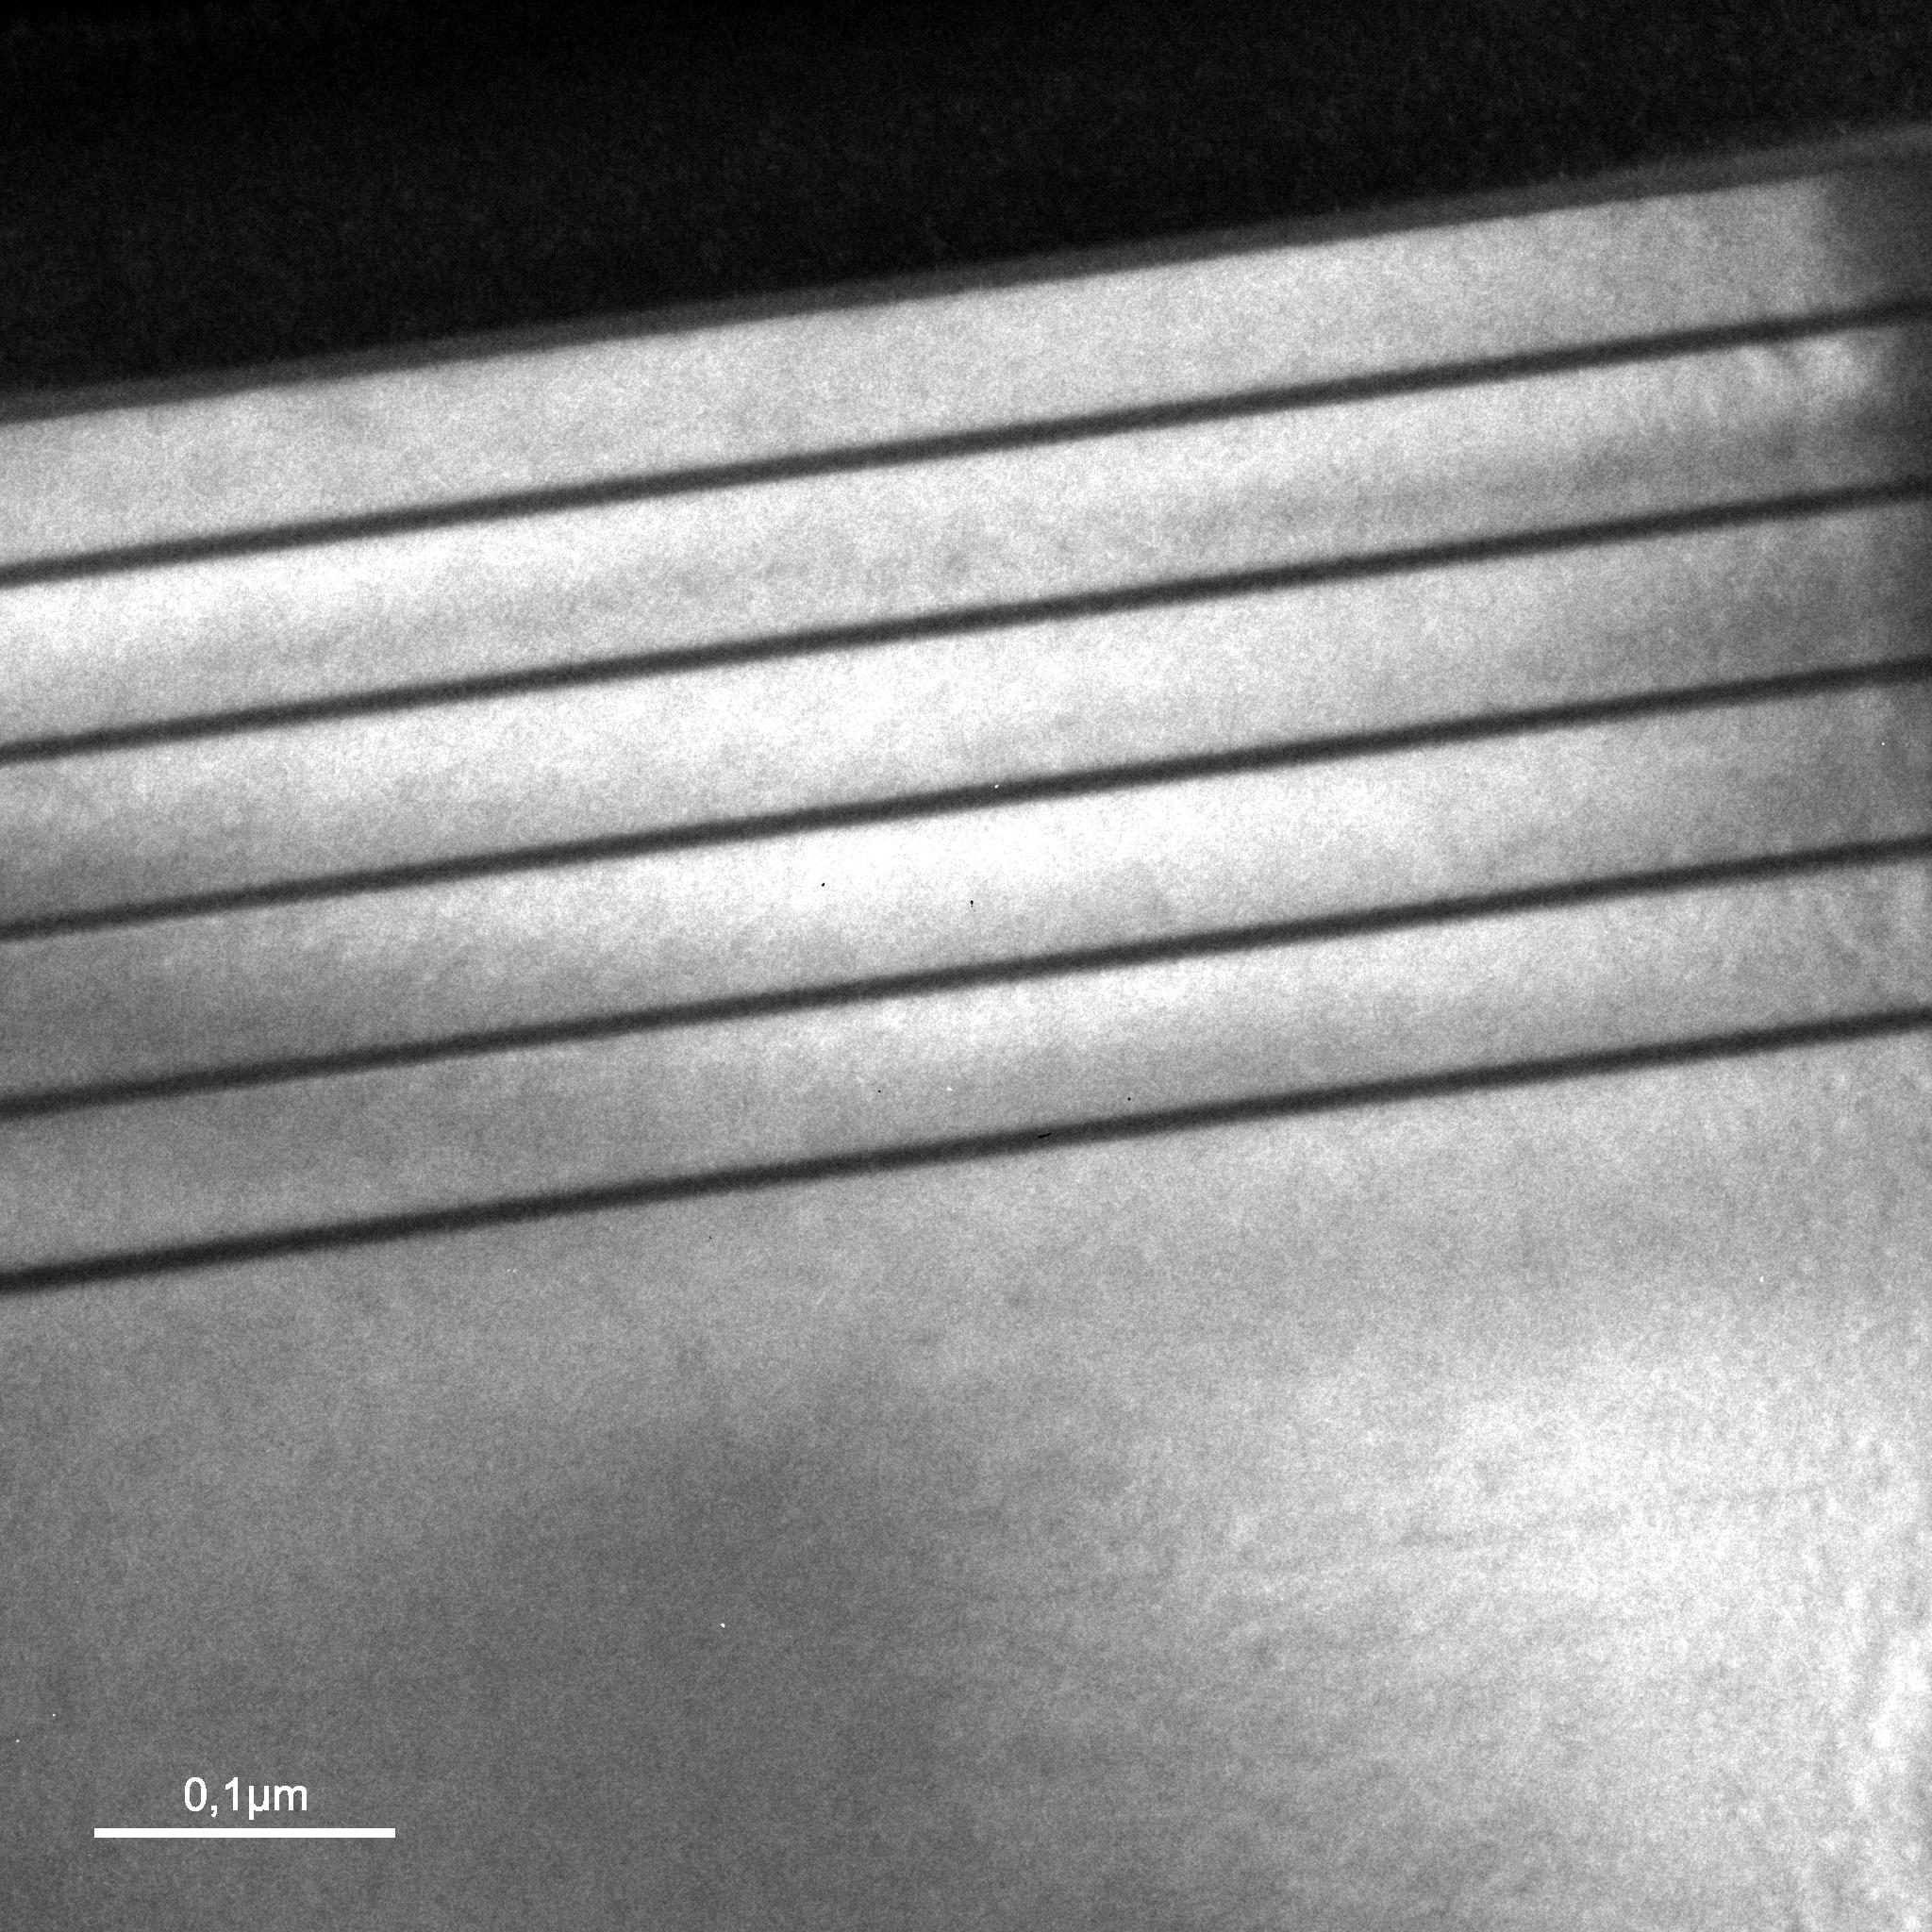
\includegraphics[width=0.49\textwidth]{Versuchsdaten/11/34000x.jpg}}
	\subcaptionbox{87000-fache Vergrößerung\label{87k}}
	[.49\linewidth]{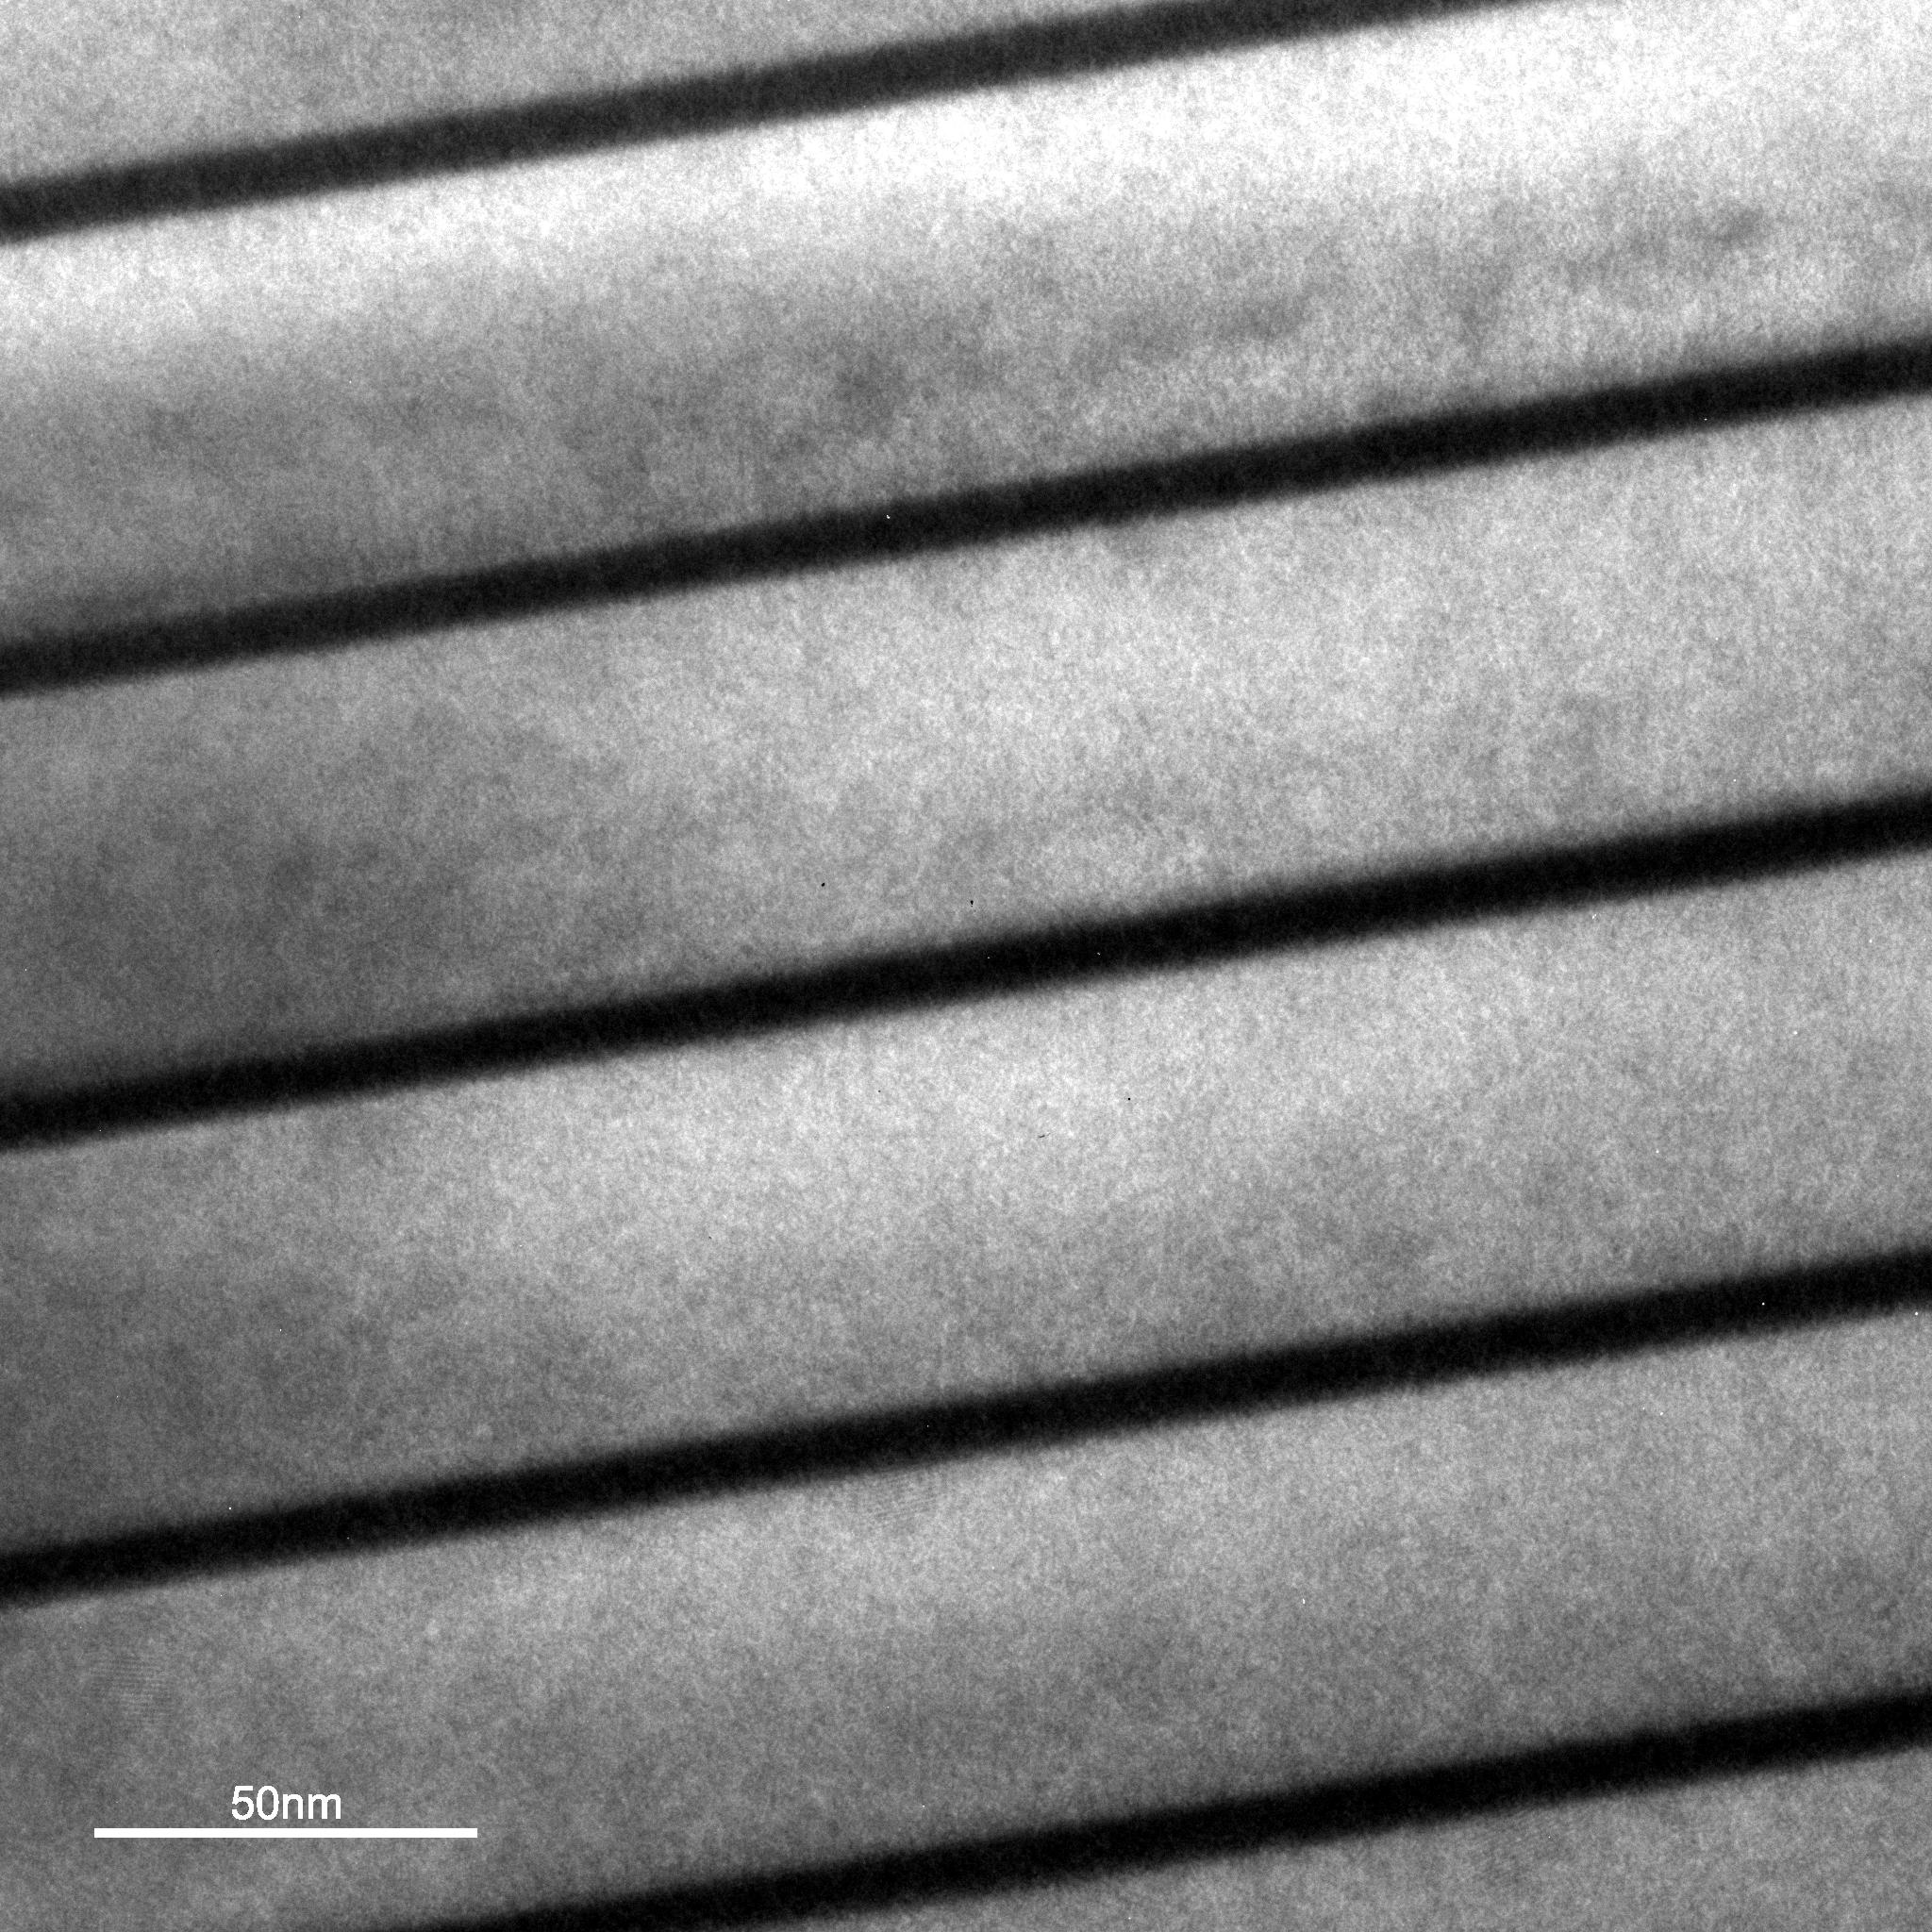
\includegraphics[width=0.49\textwidth]{Versuchsdaten/11/87000x.jpg}}\\
	\subcaptionbox{185000-fache Vergrößerung\label{185k}}
	[.49\linewidth]{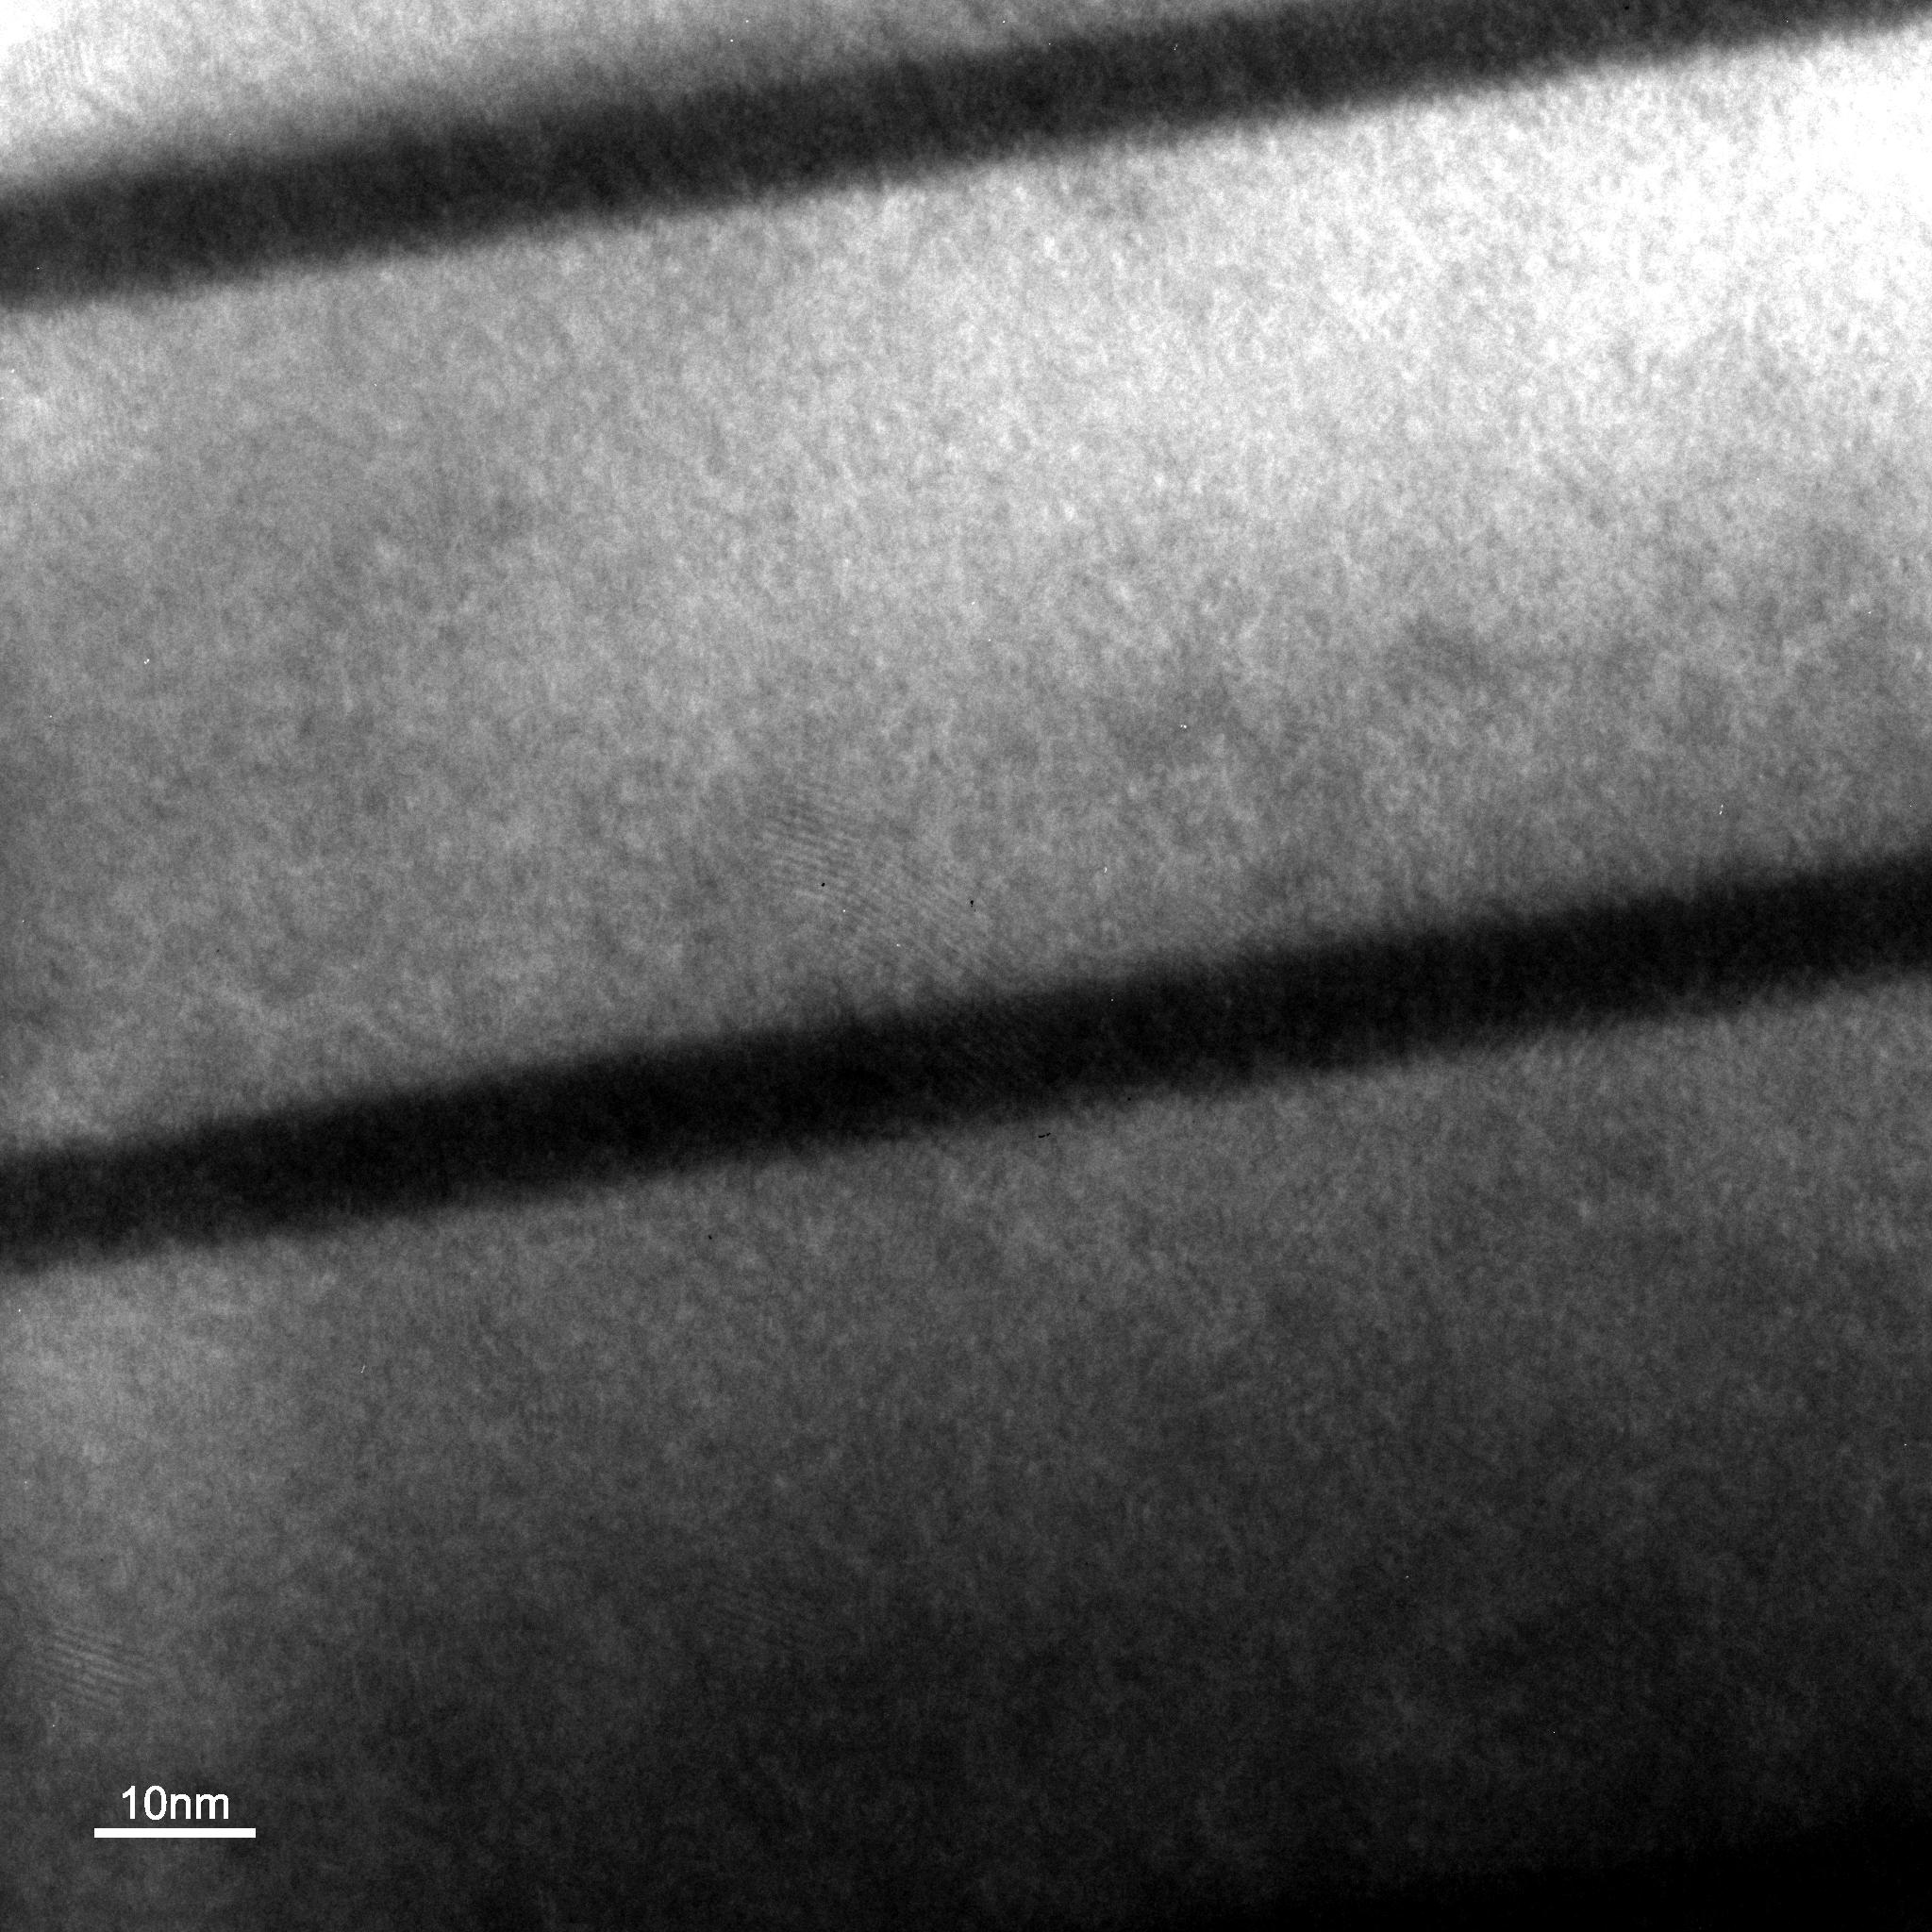
\includegraphics[width=0.49\textwidth]{Versuchsdaten/11/185000x.jpg}}
	\subcaptionbox{380000-fache Vergrößerung\label{380k}}
	[.49\linewidth]{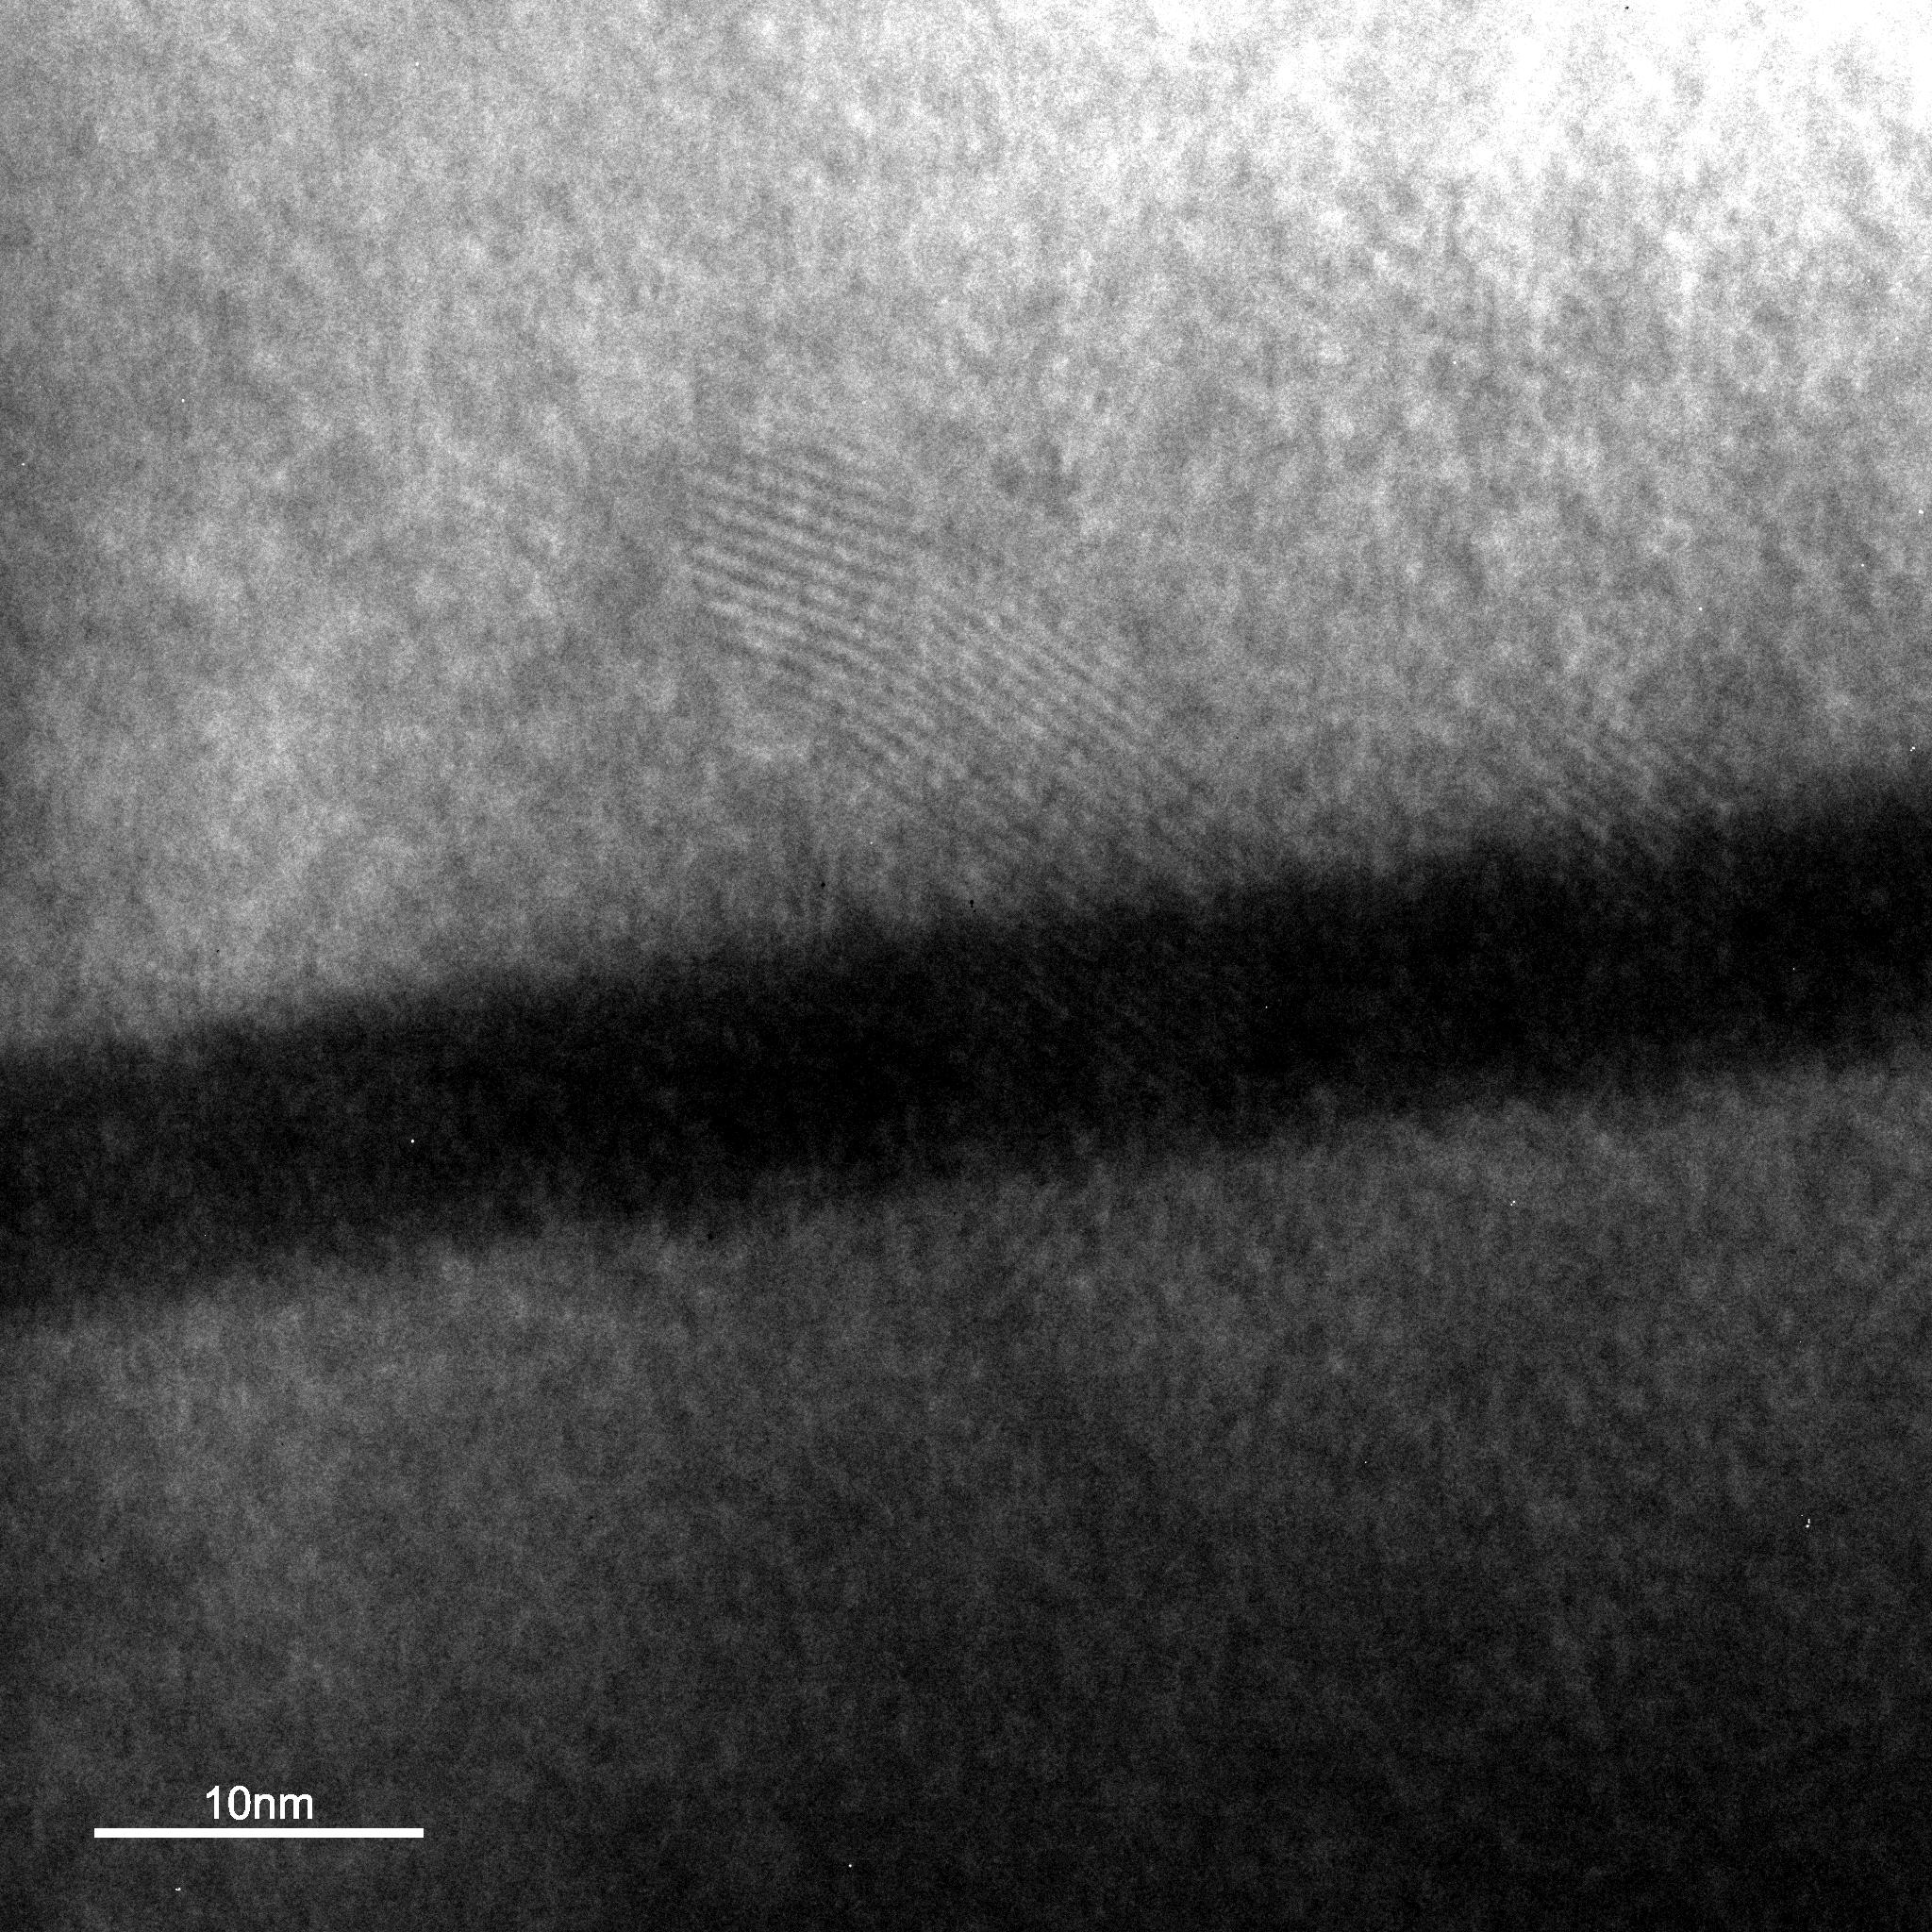
\includegraphics[width=0.49\textwidth]{Versuchsdaten/11/380000x.jpg}}
	\caption{(020) Dunkelfeldaufnahmen der InGaAs-Quantentröge mit unterschiedlichen Vergrößerungen} \label{*}
\end{figure}

\begin{figure}[htb]\centering
	\subcaptionbox{34000-fache Vergrößerung\label{34kaus}}
	[.49\linewidth]{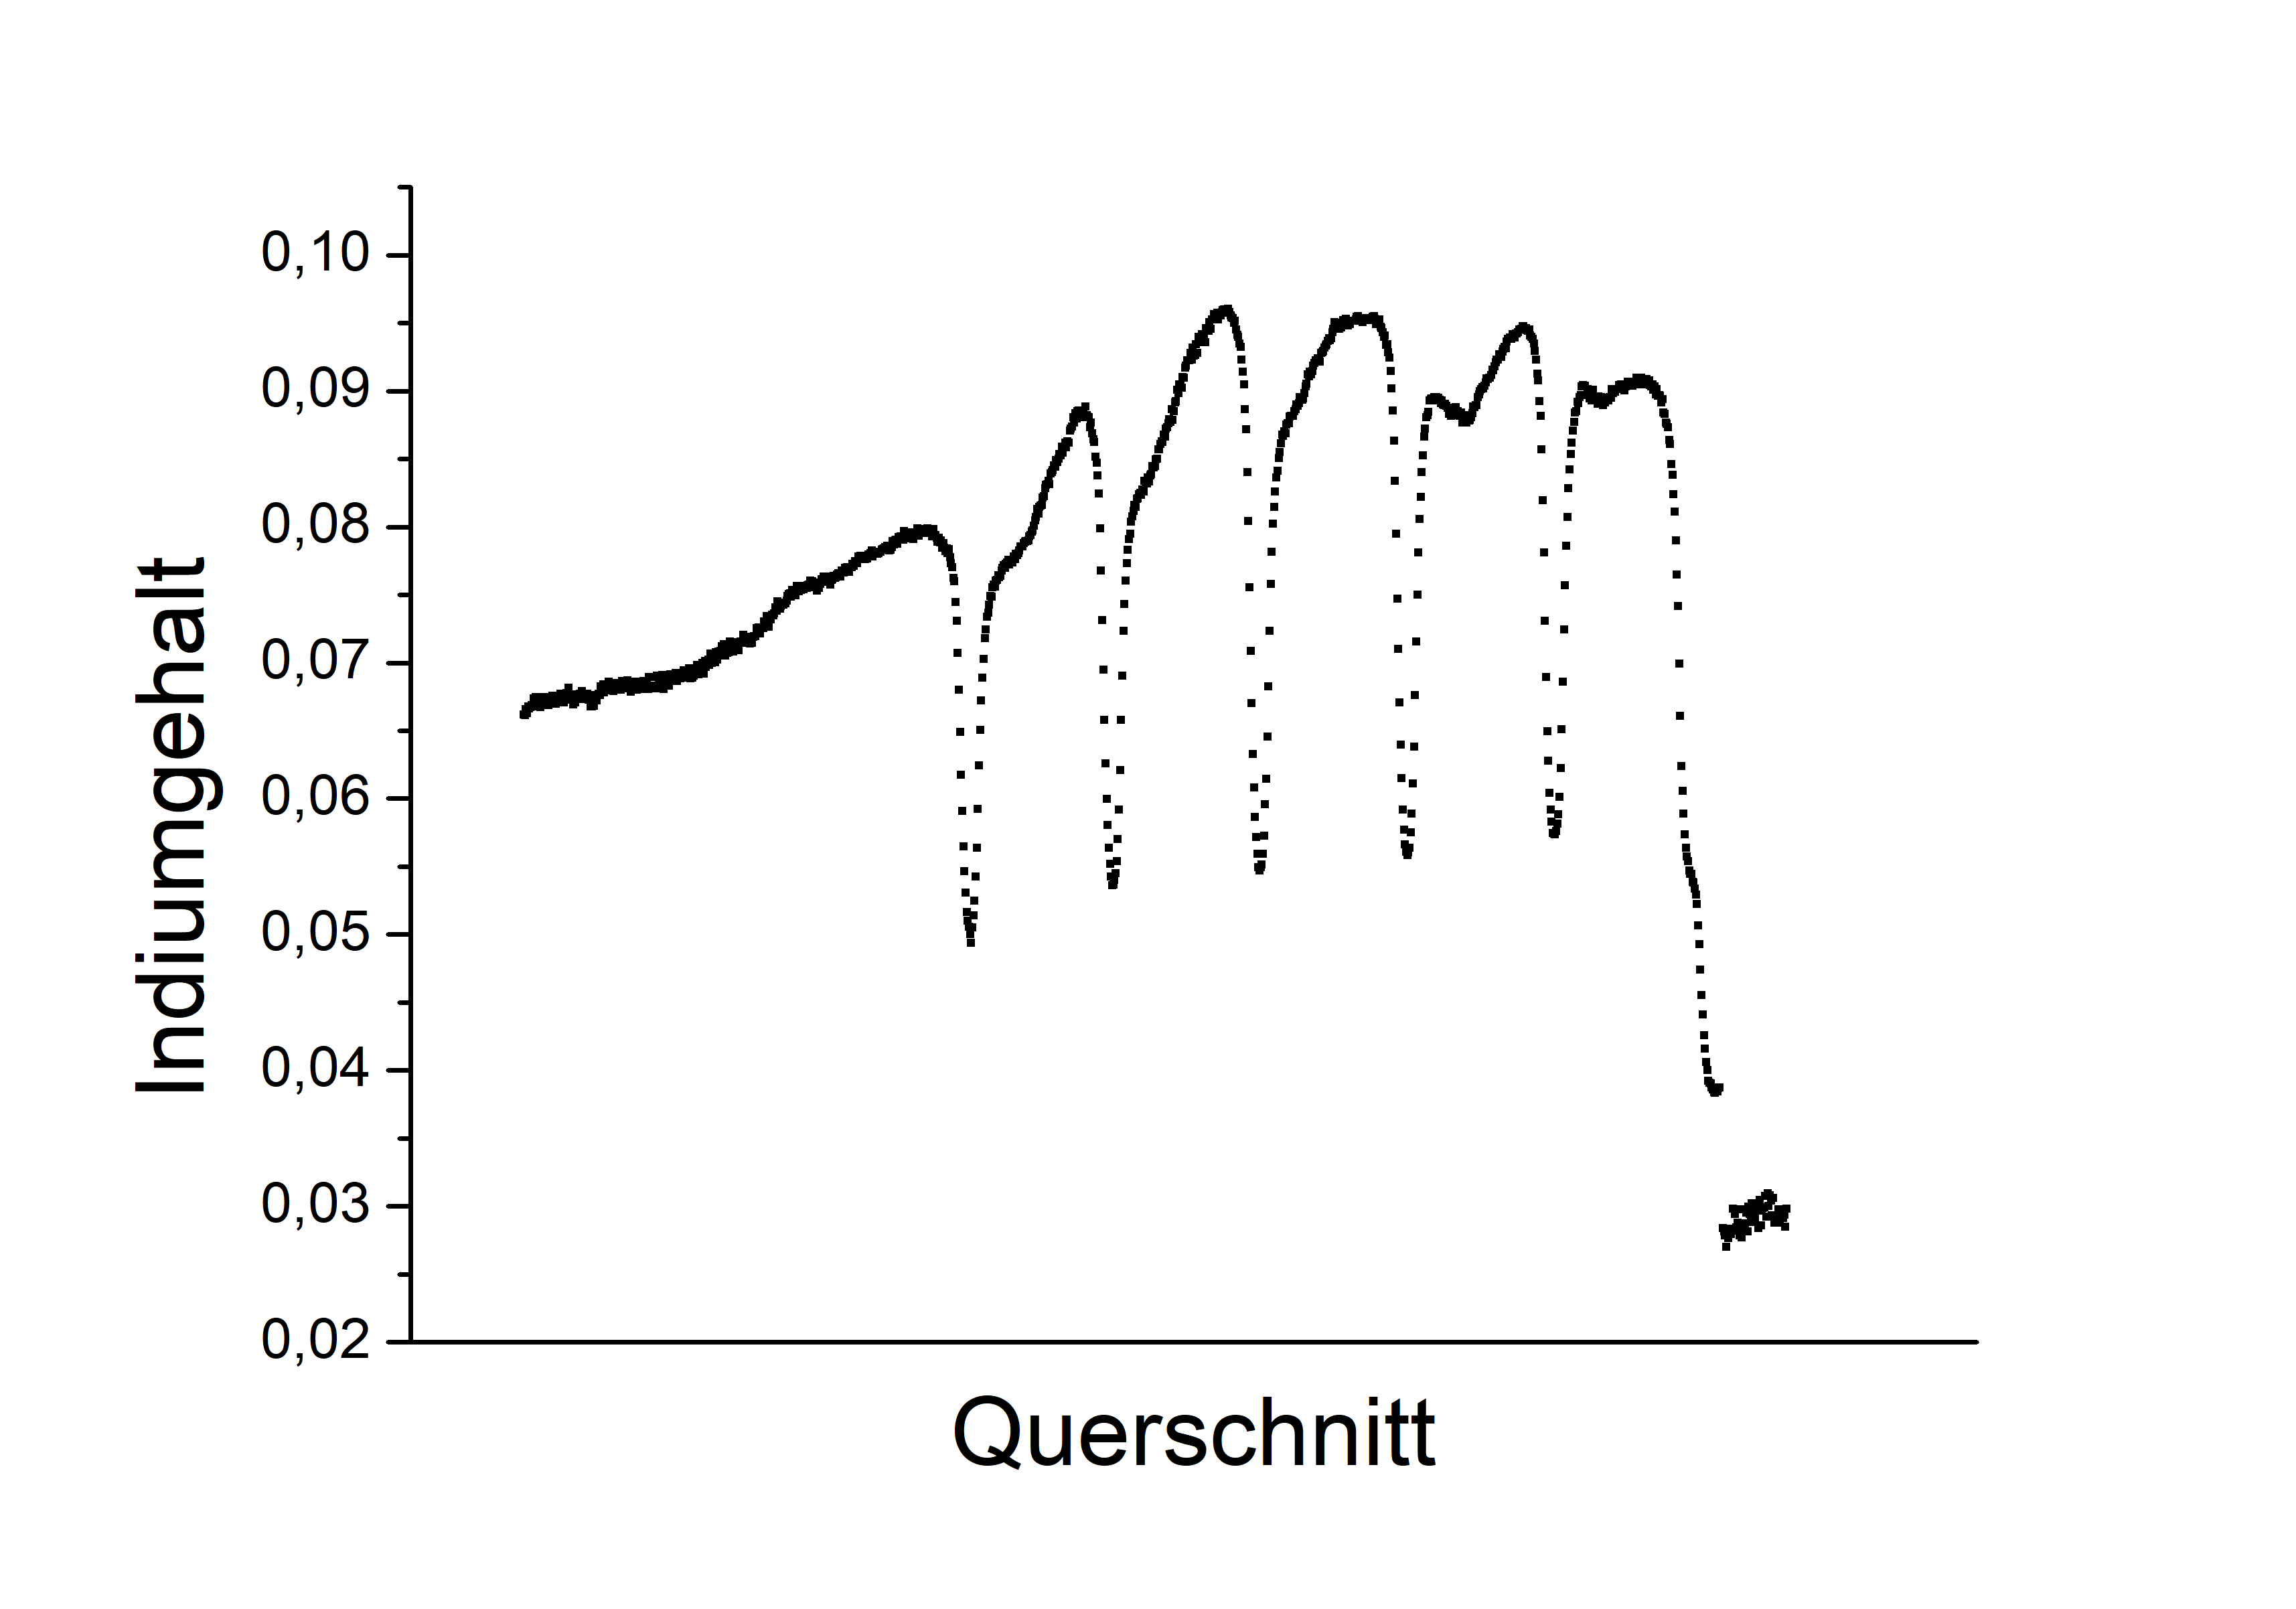
\includegraphics[width=0.49\textwidth]{Versuchsdaten/11/34000xausschnitt.png}}
	\subcaptionbox{87000-fache Vergrößerung\label{87kaus}}
	[.49\linewidth]{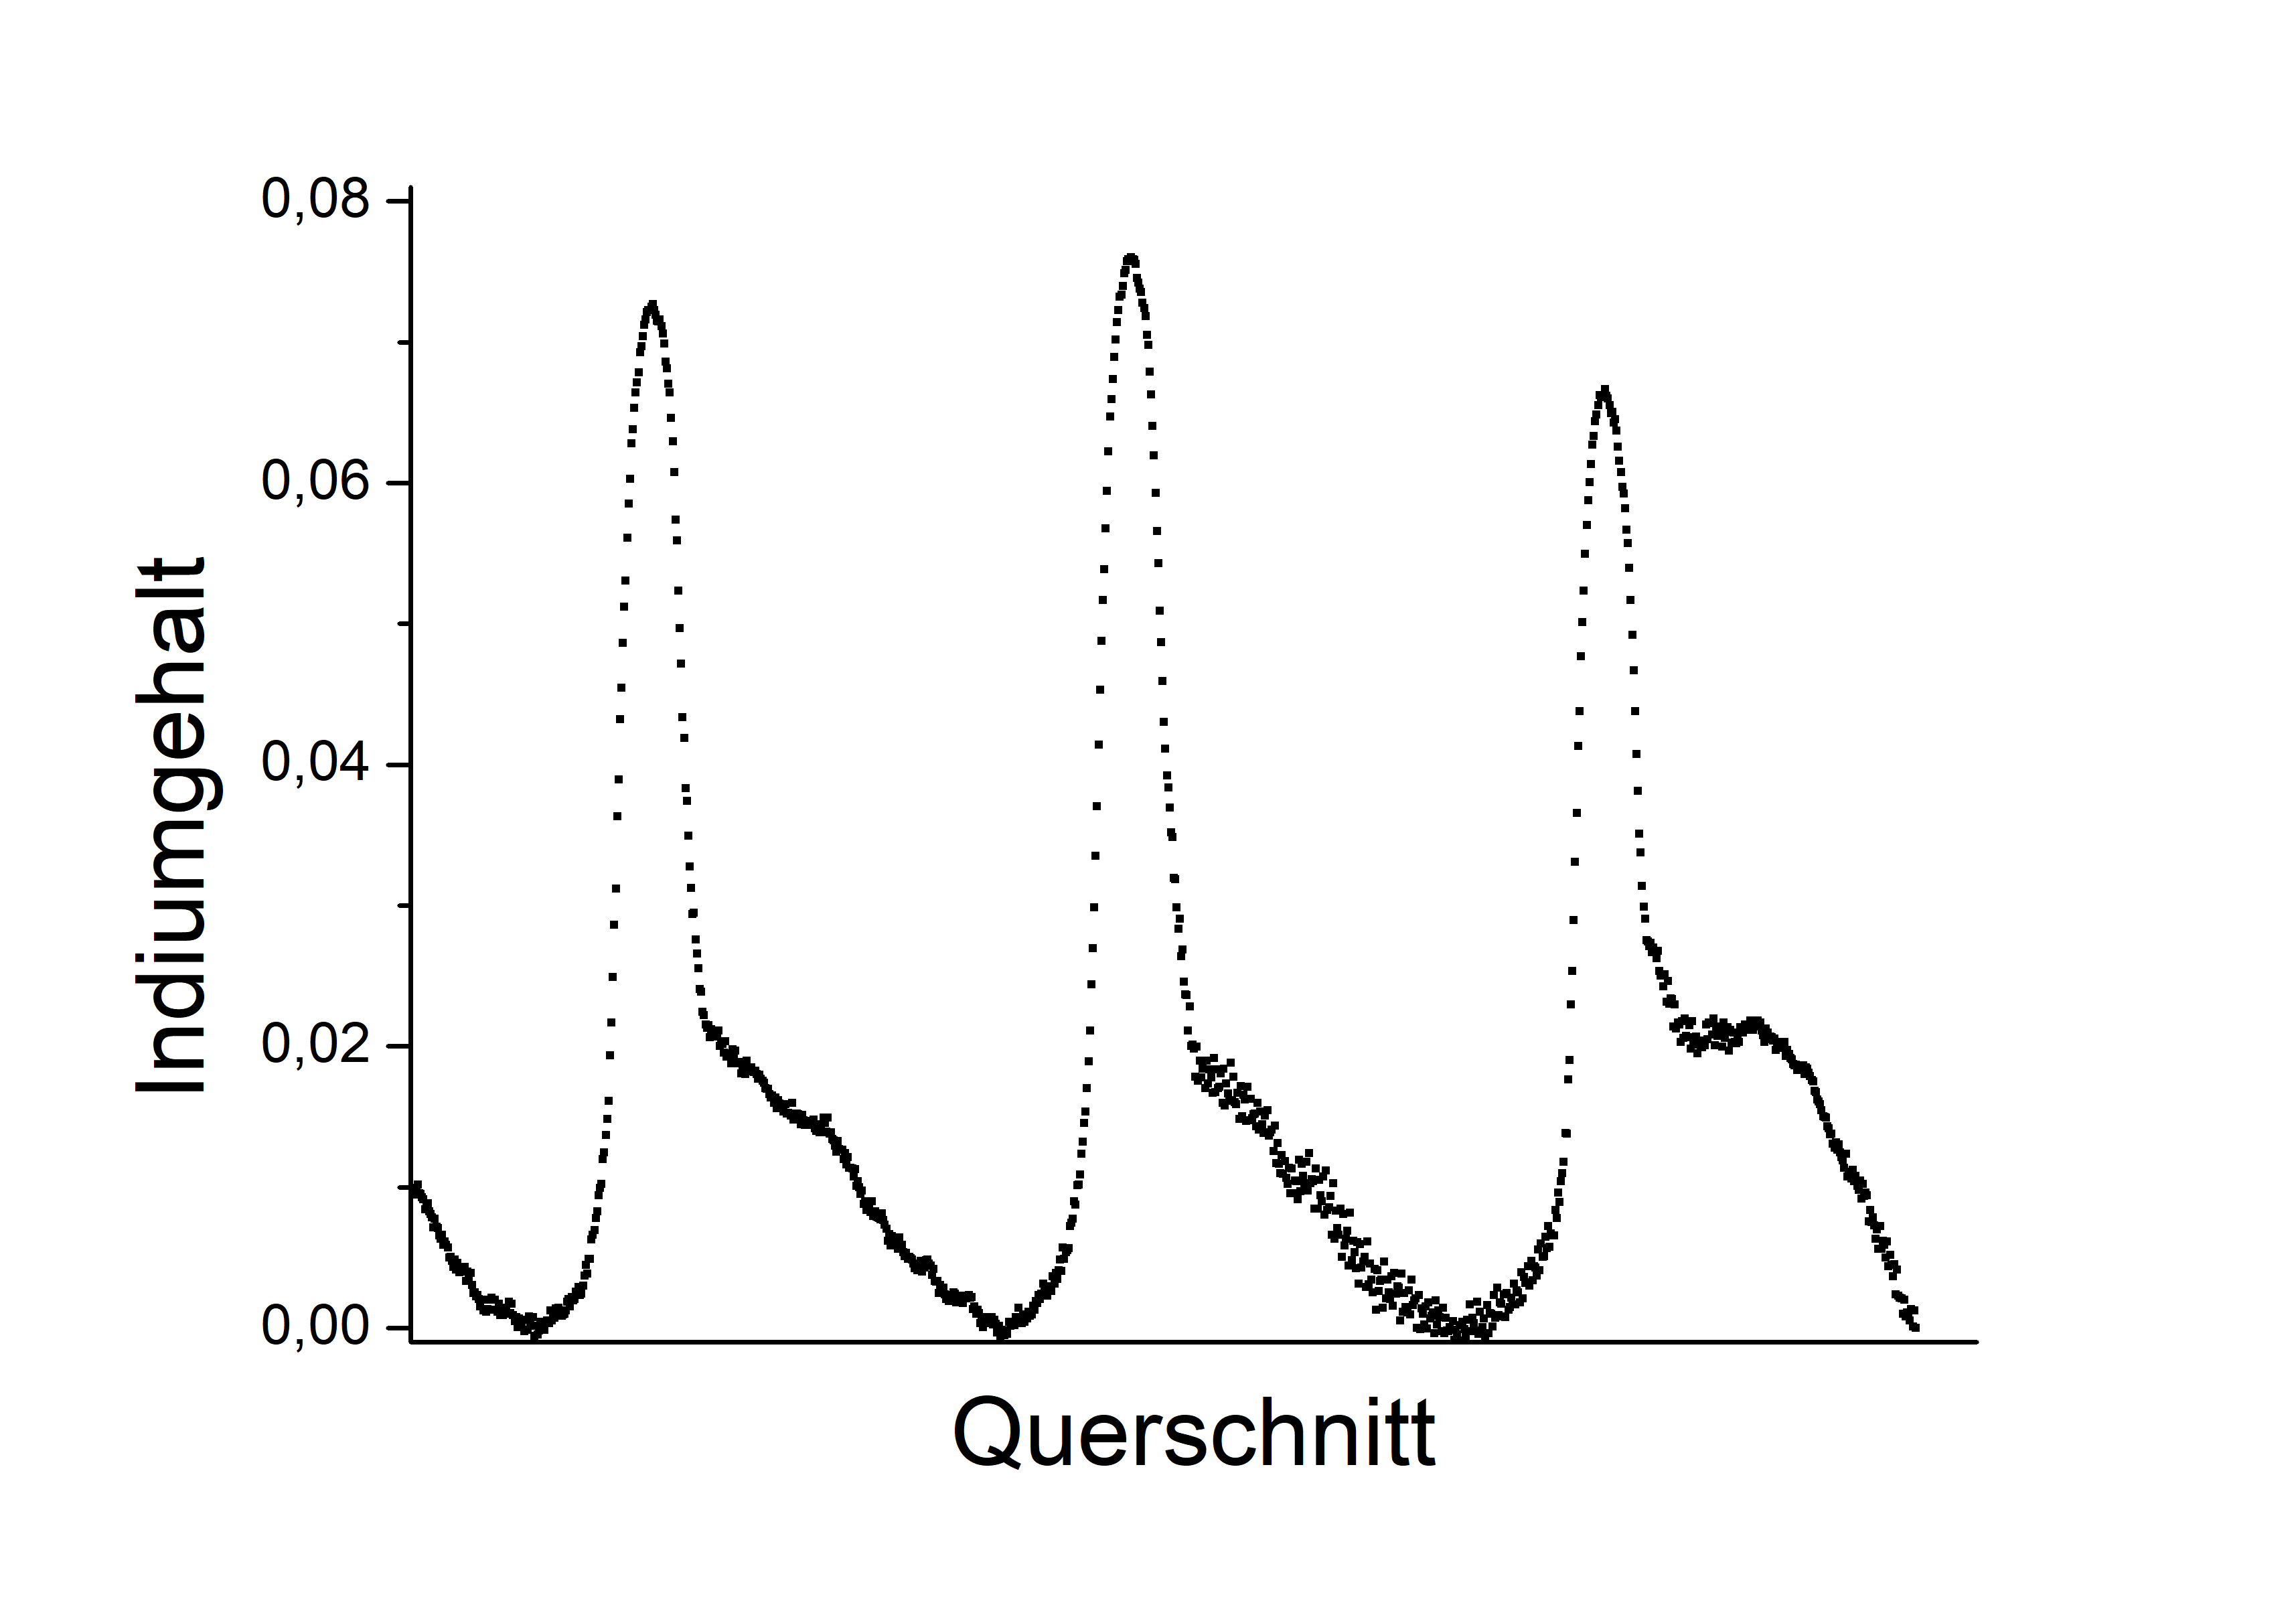
\includegraphics[width=0.49\textwidth]{Versuchsdaten/11/87000xausschnitt.png}}\\
	\subcaptionbox{185000-fache Vergrößerung\label{185kaus}}
	[.49\linewidth]{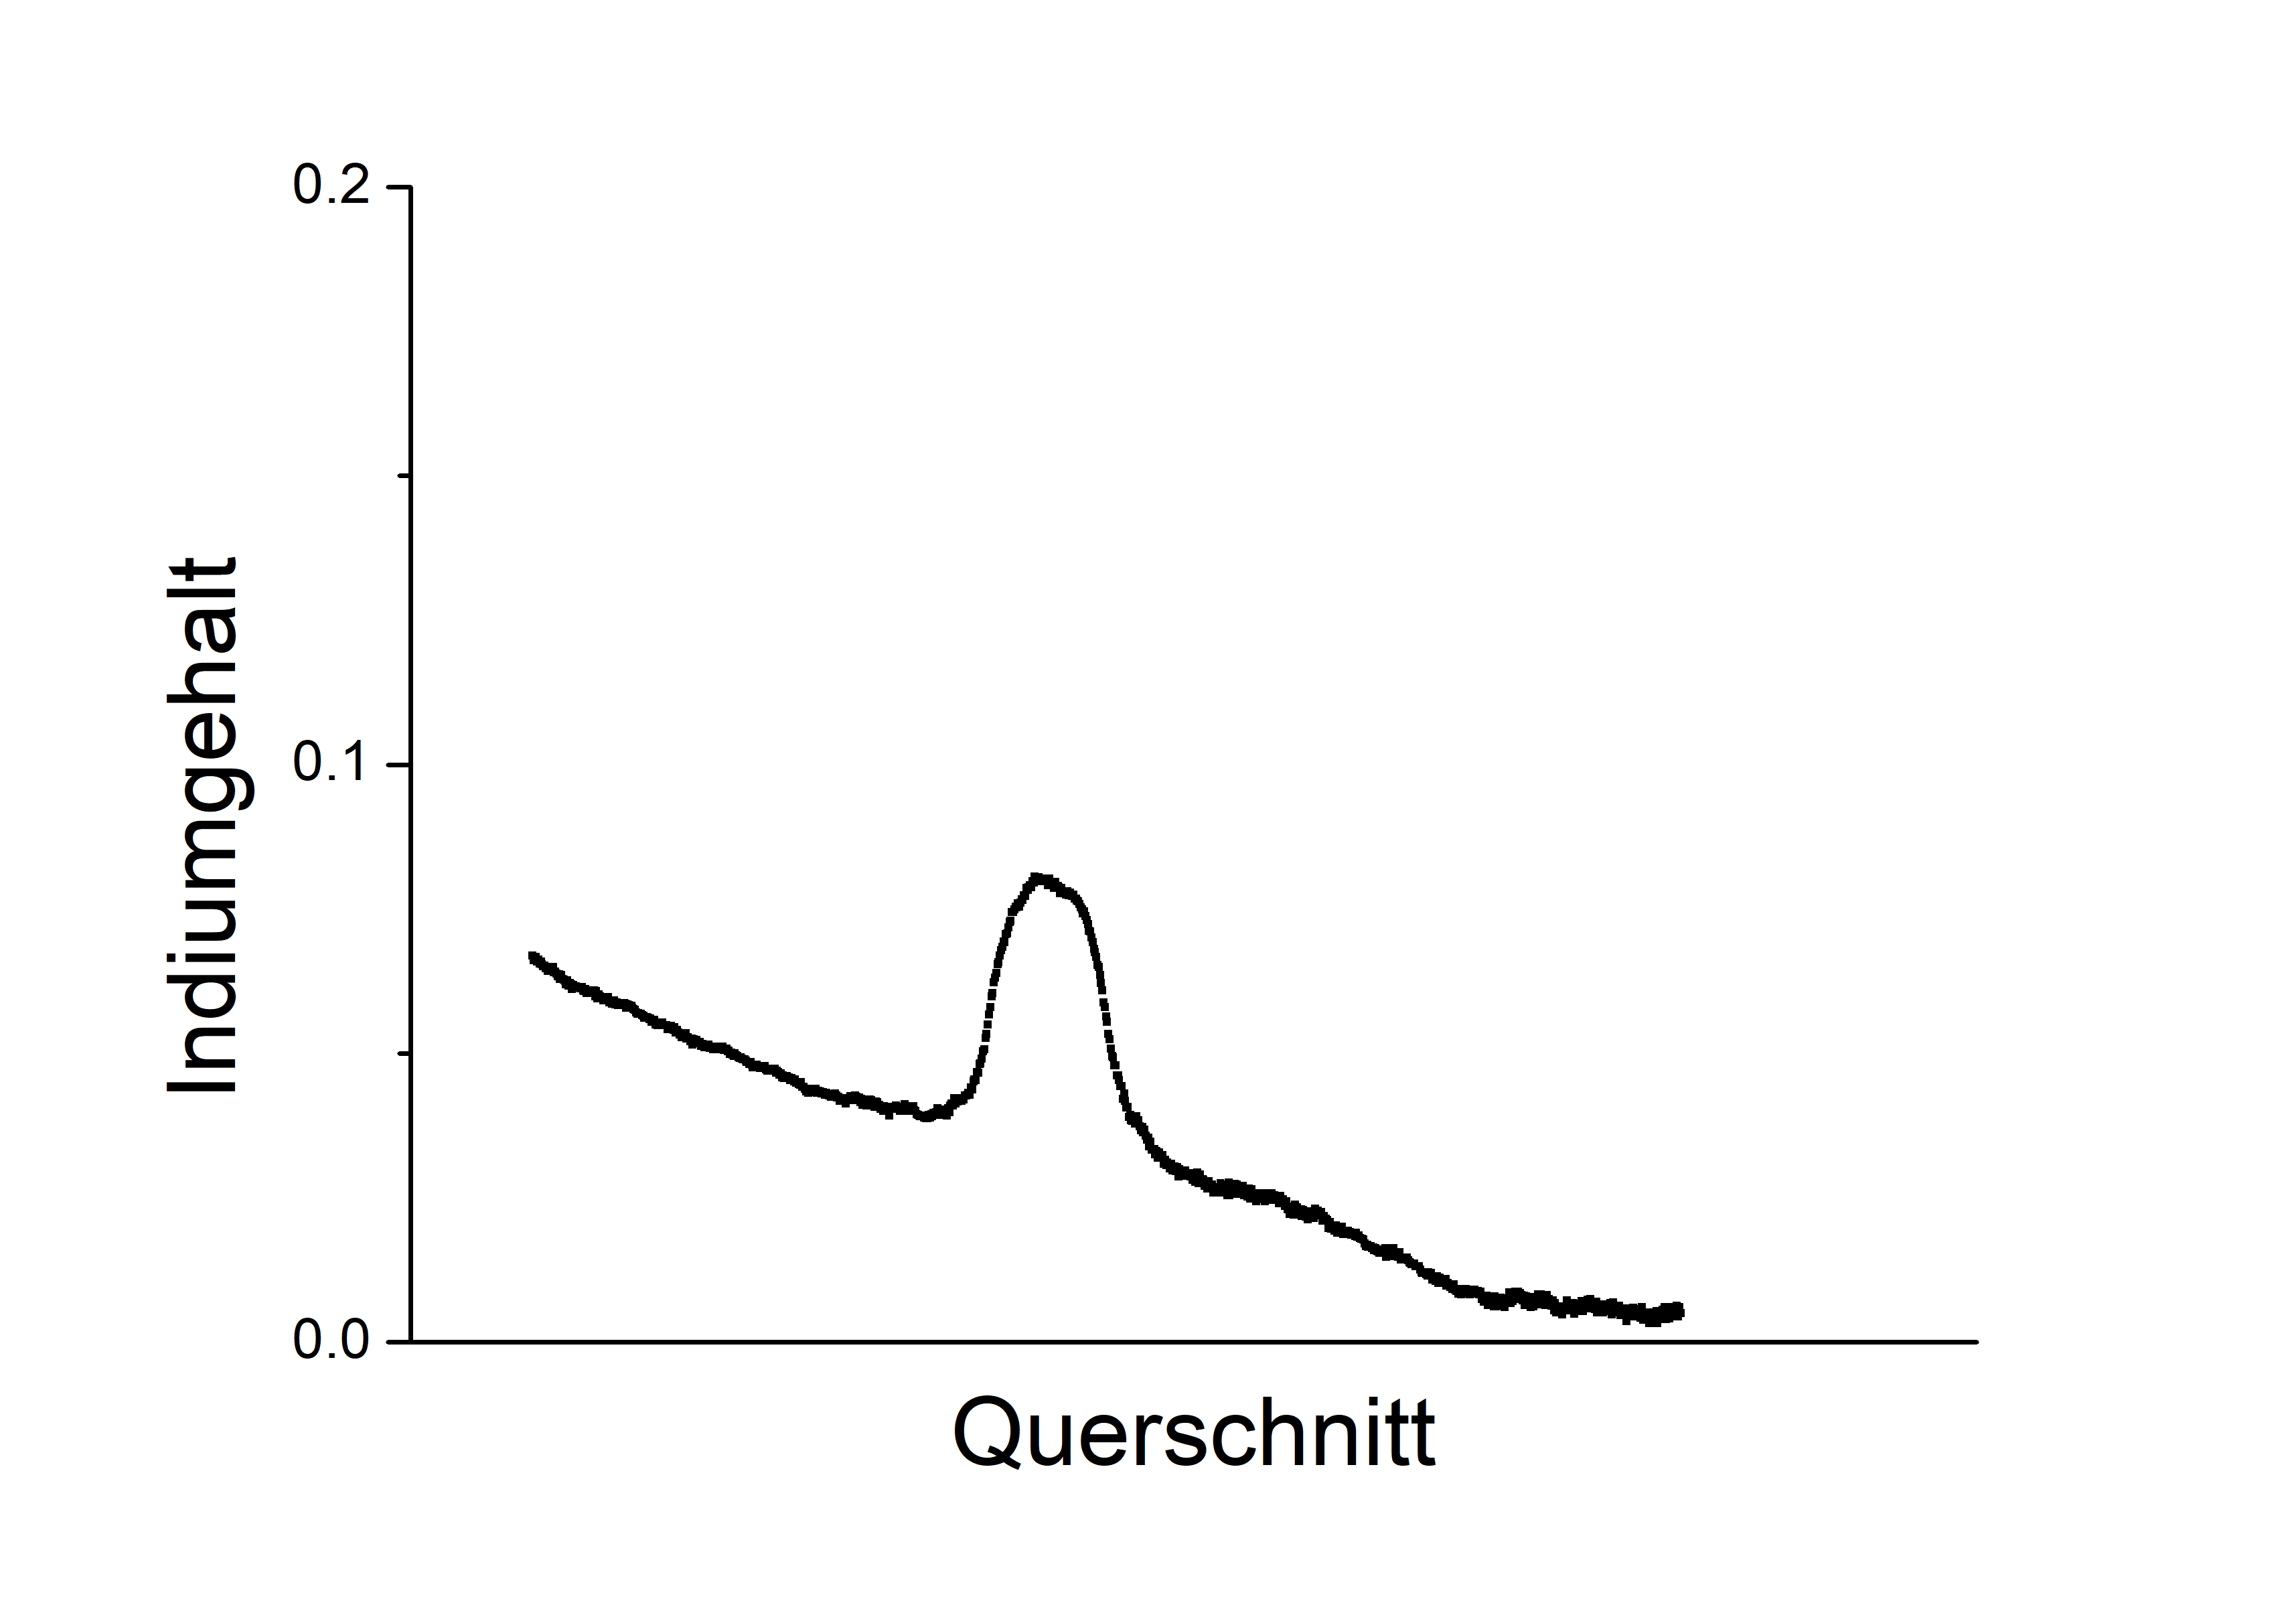
\includegraphics[width=0.49\textwidth]{Versuchsdaten/11/185000xausschnitt.png}}
	\subcaptionbox{380000-fache Vergrößerung\label{380kaus}}
	[.49\linewidth]{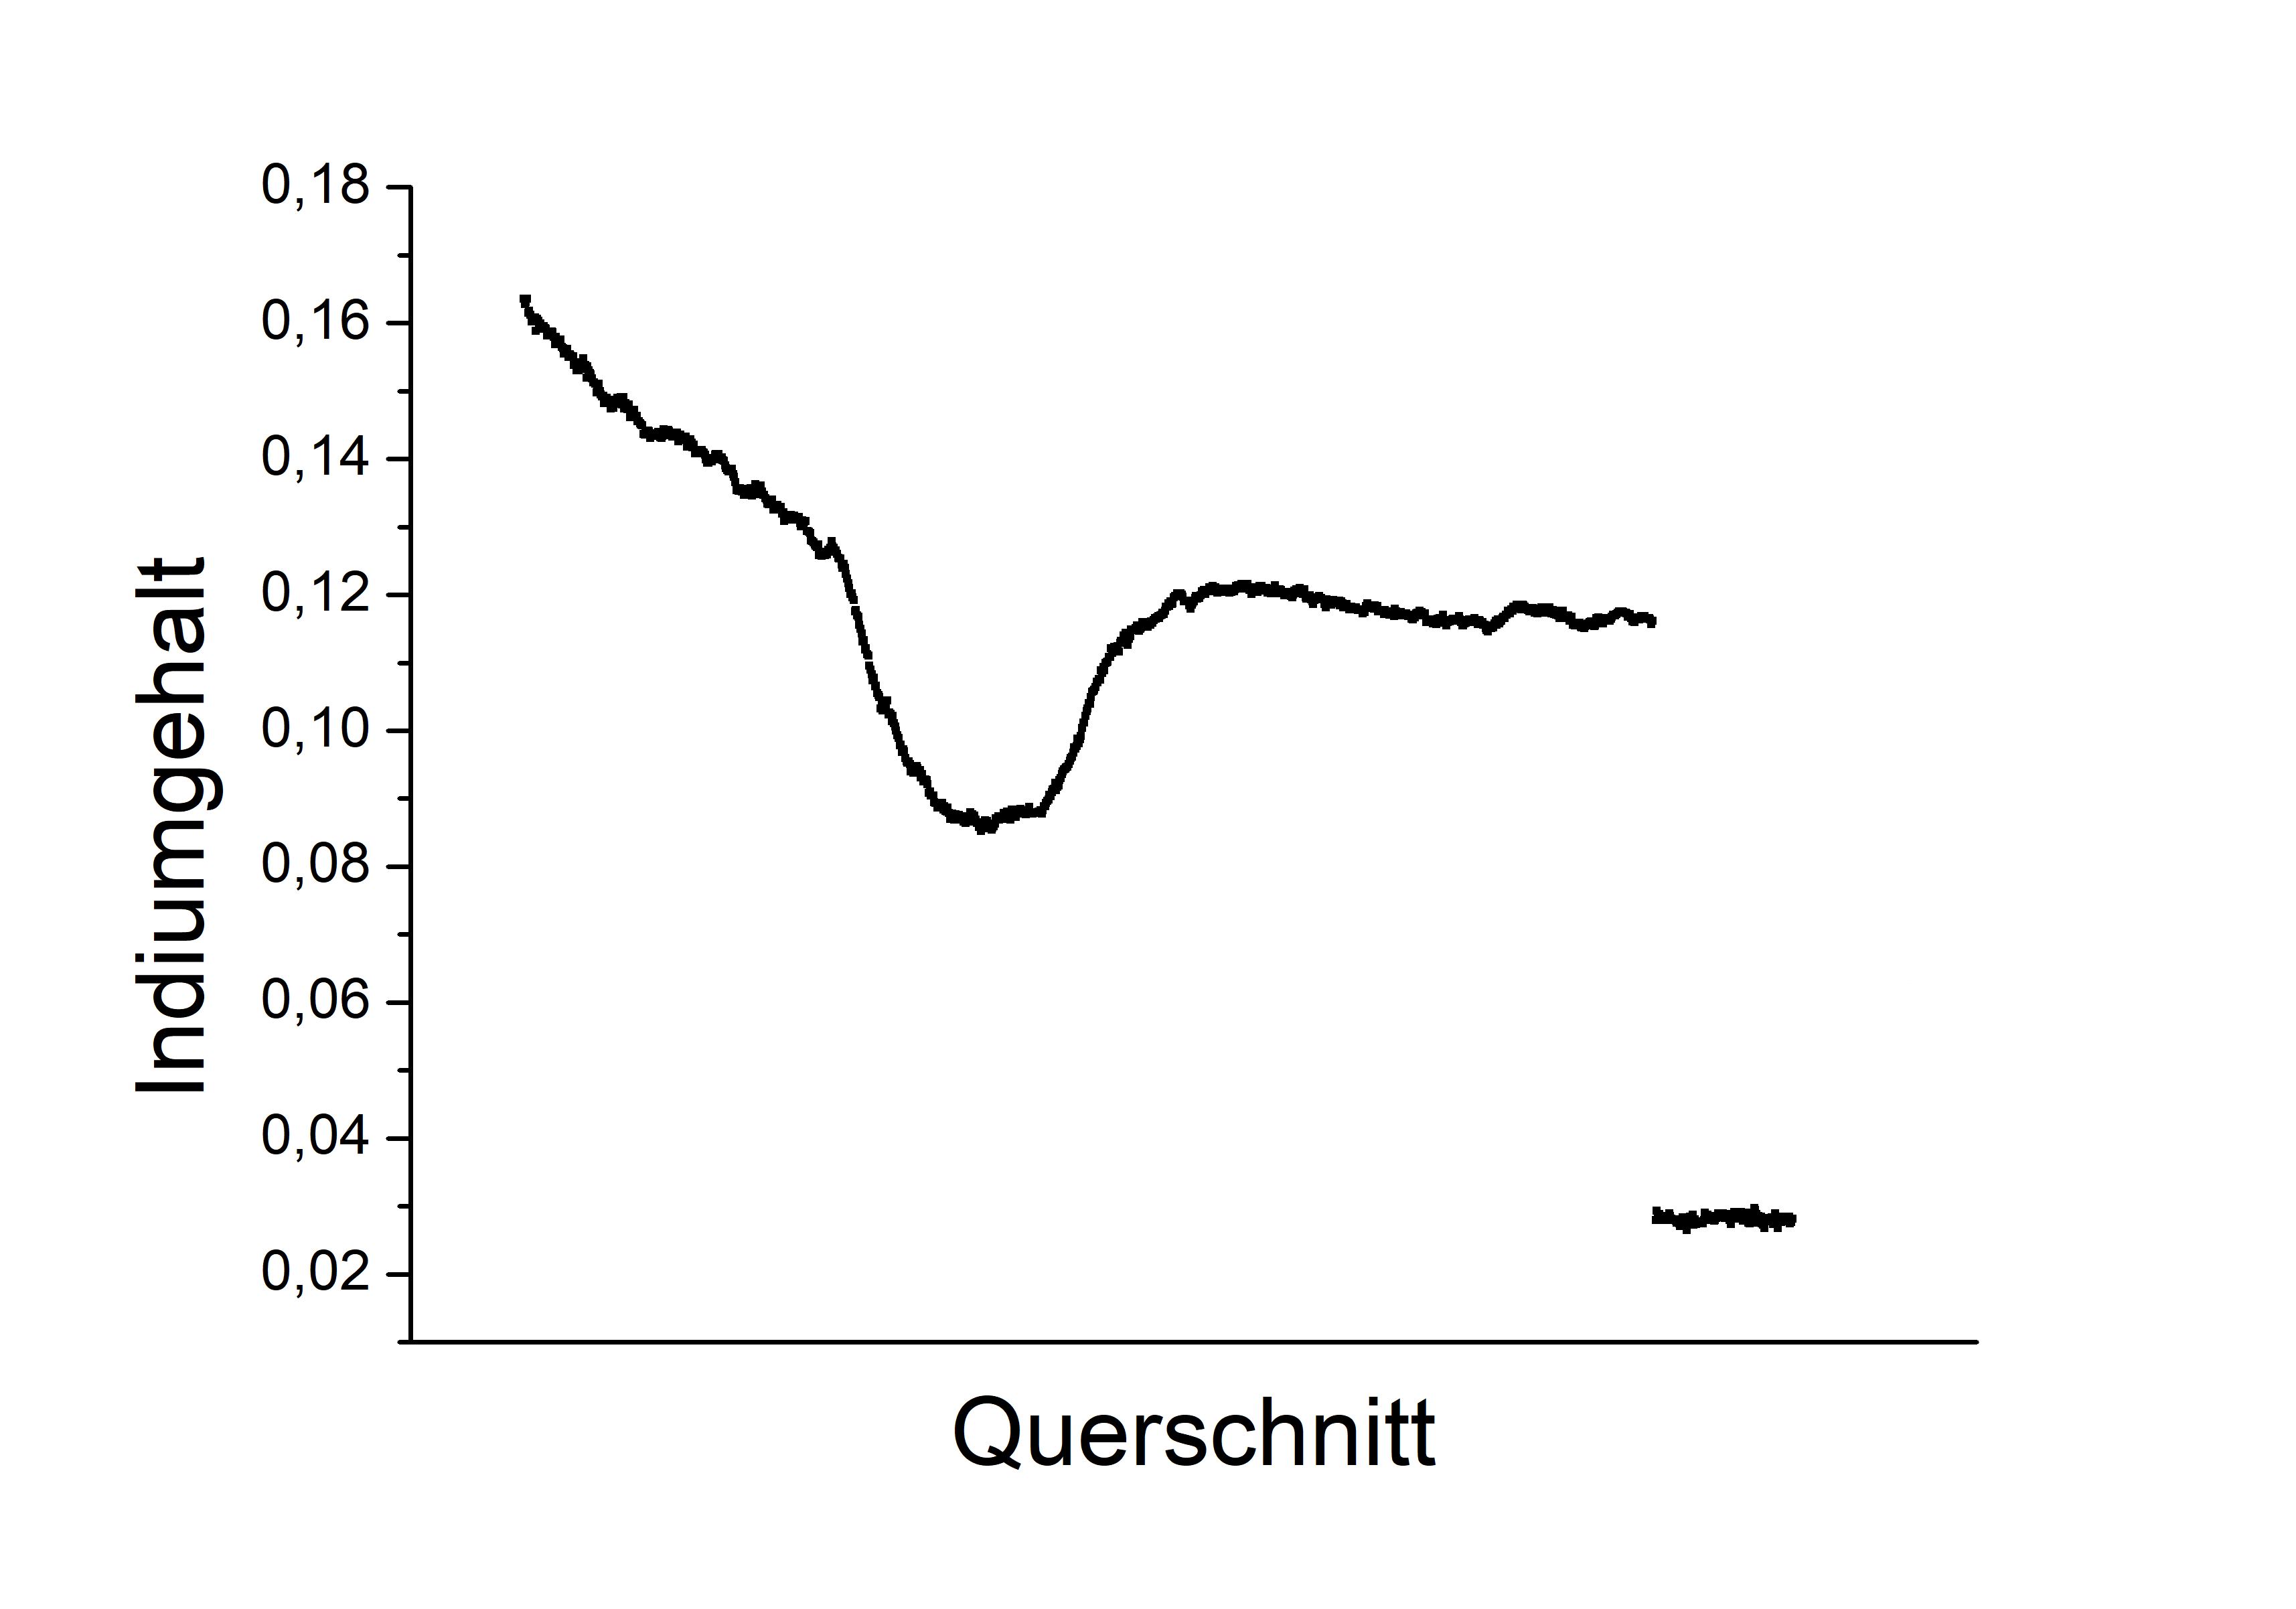
\includegraphics[width=0.49\textwidth]{Versuchsdaten/11/380000xausschnitt.png}}
	\caption{Indiumgehalt der Ausschnitte im Querschnitt} \label{ausschnitte}
\end{figure}

\section{Zusammenfassung}

\section*{Anhang}

\end{document}